%
% Main document
% ===========================================================================
% This is part of the document "Project documentation template".
% Authors: brd3
%

%---------------------------------------------------------------------------
\documentclass[
	a4paper,					% paper format
	10pt,							% fontsize
	twoside,					% double-sided
	openright,				% begin new chapter on right side
	notitlepage,			% use no standard title page
	parskip=half,			% set paragraph skip to half of a line
]{scrreprt}					% KOMA-script report
%---------------------------------------------------------------------------

\raggedbottom
\KOMAoptions{cleardoublepage=plain}			% Add header and footer on blank pages


% Load Standard Packages:
%---------------------------------------------------------------------------
\usepackage[standard-baselineskips]{cmbright}

\usepackage[ngerman]{babel}										% german hyphenation
%\usepackage[latin1]{inputenc}  							% Unix/Linux - load extended character set (ISO 8859-1)
\usepackage[ansinew]{inputenc}  							% Windows - load extended character set (ISO 8859-1)
\usepackage[T1]{fontenc}											% hyphenation of words with �,� and �
\usepackage{textcomp}													% additional symbols
\usepackage{ae}																% better resolution of Type1-Fonts 
\usepackage{fancyhdr}													% simple manipulation of header and footer 
\usepackage{graphicx}                      		% integration of images
\usepackage{float}														% floating objects
\usepackage{caption}													% for captions of figures and tables
\usepackage{booktabs}													% package for nicer tables
\usepackage{tocvsec2}													% provides means of controlling the sectional numbering
\usepackage{color}
\usepackage{fancyvrb}
\usepackage{listings}
\usepackage{titleref}

%---------------------------------------------------------------------------

% Load Math Packages
%---------------------------------------------------------------------------
\usepackage{amsmath}                    	   	% various features to facilitate writing math formulas
\usepackage{amsthm}                       	 	% enhanced version of latex's newtheorem
\usepackage{amsfonts}                      		% set of miscellaneous TeX fonts that augment the standard CM
\usepackage{amssymb}													% mathematical special characters
\usepackage{exscale}													% mathematical size corresponds to textsize
%---------------------------------------------------------------------------

% Package to facilitate placement of boxes at absolute positions
%---------------------------------------------------------------------------
\usepackage[absolute]{textpos}
\setlength{\TPHorizModule}{1mm}
\setlength{\TPVertModule}{1mm}
%---------------------------------------------------------------------------					
			
% Definition of Colors
%---------------------------------------------------------------------------
\RequirePackage{color}                          % Color (not xcolor!)
\definecolor{linkblue}{rgb}{0,0,0.8}            % Standard
\definecolor{darkblue}{rgb}{0,0.08,0.45}        % Dark blue
\definecolor{brickred}{cmyk}{0,0.89,0.94,0.28}  % Brickred
%\definecolor{linkcolor}{rgb}{0,0,0.8}     			% Blue for the web- and cd-version!
\definecolor{linkcolor}{rgb}{0,0,0}        			% Black for the print-version!
\definecolor{bfhred}{rgb}{0.776,0,0.066}  			% Red
\definecolor{commentgreen}{rgb}{0,0.5,0}  % Green for java comments
%---------------------------------------------------------------------------

% Hyperref Package (Create links in a pdf)
%---------------------------------------------------------------------------
\usepackage[
	pdftex,ngerman,bookmarks,plainpages=false,pdfpagelabels,
	backref = {false},										% No index backreference
	colorlinks = {true},                  % Color links in a PDF
	hypertexnames = {true},               % no failures "same page(i)"
	bookmarksopen = {true},               % opens the bar on the left side
	bookmarksopenlevel = {0},             % depth of opened bookmarks
	pdftitle = {Bachelor Thesis - AI Bot f�r Computerspiele},	   	% PDF-property
	pdfauthor = {kases1 kustl1},        					  % PDF-property
	pdfsubject = {Documentation},        % PDF-property
	linkcolor = {linkcolor},              % Color of Links
	citecolor = {linkcolor},              % Color of Cite-Links
	urlcolor = {linkcolor},               % Color of URLs
]{hyperref}
%---------------------------------------------------------------------------
 
\lstset{fancyvrb=true}
\lstset{
basicstyle=\small\tt,
keywordstyle=\color{darkblue},
identifierstyle=,
commentstyle=\color{commentgreen},
stringstyle=\color{brickred},
showstringspaces=false,
tabsize=3,
captionpos=b,
numberstyle=\tiny,
breaklines=true
%stepnumber=4
}
% Set up page dimension
%---------------------------------------------------------------------------
\usepackage{geometry}
\geometry{
	a4paper,
	left=28mm,
	right=15mm,
	top=30mm,
	headheight=20mm,
	headsep=10mm,
	textheight=242mm,
	footskip=15mm
}
%---------------------------------------------------------------------------

% Makeindex Package
%---------------------------------------------------------------------------
\usepackage{makeidx}                         		% To produce index
\makeindex                                    	% Index-Initialisation
%---------------------------------------------------------------------------

% Glossary Package
%---------------------------------------------------------------------------
% the glossaries package uses makeindex
% if you use TeXnicCenter do the following steps:
%  - Goto "Ausgabeprofile definieren" (ctrl + F7)
%  - Select the profile "LaTeX => PDF"
%  - Add in register "Nachbearbeitung" a new "Postprozessoren" point named Glossar
%  - Select makeindex.exe in the field "Anwendung" ( ..\MiKTeX x.x\miktex\bin\makeindex.exe )
%  - Add this [ -s "%tm.ist" -t "%tm.glg" -o "%tm.gls" "%tm.glo" ] in the field "Argumente"
%
% for futher informations go to http://ewus.de/tipp-1029.html
%---------------------------------------------------------------------------
\usepackage[nonumberlist]{glossaries}
\makeglossaries
\newglossaryentry{Tile}{name={Tile},description={Ortsangabe auf dem Spielfeld mit Row (Zeile) und Column (Spalte) beschrieben. Bsp: <r:12 c:10>}}
\newglossaryentry{FogofWar}{name={Fog of War},description={Teil der Karte, der durch die eigenen Einheiten nicht mehr sichtbar ist}}
\newglossaryentry{AI}{name={AI},description={Artificial Intelligence - K�nstliche Intelligenz}}
\newglossaryentry{Bot}{name={Bot},description={AI-Agent f�r ein Computerspiel}}
\newglossaryentry{API}{name={API},description={Application Programming Interface - Programmierschnittstelle}}
\newglossaryentry{InfluenceMap}{name={Influence Map},description={Datenstruktur, die zur Berechnung des Einflusses von Spieleinheiten auf die Spielkarte dient}}
\newglossaryentry{LazyInitialization}{name={Lazy Initialization},description={Bei der Lazy Initialization wird eine Ressource erst beim erstmaligen Gebrauch initialisiert (z.B. ein Logfile erst mit dem ersten Log-Eintrag erstellt)}}

%---------------------------------------------------------------------------

% Intro:
%---------------------------------------------------------------------------
\begin{document}                              	% Start Document
\settocdepth{subsubsection}																	% Set depth of toc
\pagenumbering{roman}														
%---------------------------------------------------------------------------

% Set up header and footer
%---------------------------------------------------------------------------
\fancyhf{}																		% clean all fields
\fancypagestyle{plain}{												% new definition of plain style
	\fancyfoot[OR,EL]{\footnotesize \thepage} 	% footer right part --> page number
	\fancyfoot[OL,ER]{\footnotesize \leftmark}	% footer left part -->	chapter
	\fancyhead[C]{															% header center part --> BFH logo
		\begin{textblock}{0}[0,0](86,9)
			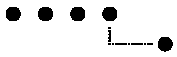
\includegraphics[scale=1.0]{91_bilder/bfh_de_without_text.pdf}
		\end{textblock}
	}
}

\renewcommand{\chaptermark}[1]{\markboth{\thechapter.  #1}{}}
\renewcommand{\headrulewidth}{0pt}				% no header stripline
\renewcommand{\footrulewidth}{0pt} 				% no bottom stripline

\pagestyle{plain}
%---------------------------------------------------------------------------

\setcounter{secnumdepth}{3}
\setcounter{tocdepth}{3}
% Title Page and Abstract
%---------------------------------------------------------------------------
%
% Project documentation template
% ===========================================================================
% This is part of the document "Project documentation template".
% Authors: brd3
%

\begin{titlepage}


% Red Bar and BFH-Logo absolute placed at (87,10) on A4
% Actually not a realy satisfactory solution but working.
%---------------------------------------------------------------------------
\setlength{\unitlength}{1mm}
\begin{textblock}{210}(-10,-10)
	\begin{picture}(210,32)
		\put(0,0){\color{bfhred}\rule{240mm}{30mm}}
	\end{picture}
\end{textblock}

\begin{textblock}{0}[0,0](84,7)
	
\includegraphics[scale=1.0]{90_bilder/bfh_de_white.pdf}
\end{textblock}

% Titel / Untertitel / Autor:
%---------------------------------------------------------------------------
\begin{flushleft}

\vspace*{4cm}

\fontsize{12pt}{15pt}\selectfont\vspace{0.5em}
Fachbereich Technik und Informatik \\
Herbstsemester 2012

\vspace{2cm}

\fontsize{30pt}{32pt}\selectfont 
\noindent \textbf{Bachelor Thesis - AI Bot f�r Computerspiele} \\
\fontsize{20pt}{22pt}\selectfont 
\noindent \textbf{Ants AI Challenge} \\


\vspace{4cm}
\fontsize{12pt}{15pt}\selectfont
\begin{tabbing}
xxxxxxxxxxxxxxx\=xxxxxxxxxxxxxxxxxxxxxxx \kill
Studierende:	\> Lukas Kuster			\\
							\> Stefan K�ser		\\
																\\
Betreuung:	\> Dr. J�rgen Eckerle	\\
																\\
Experte:	\> Dr. Federico Fl�ckiger	\\
																\\
																\\
Datum:				\> \today					\\
Version:			\> V01.00					\\
\end{tabbing}
\end{flushleft}

%\vspace{6mm}
%\fontsize{12pt}{15pt}\selectfont
%Dieses Dokument dient als Vorlage f�r die Erstellung von Berichten nach den Richtlinien der BFH. Die Vorlage ist in \LaTeX{} %erstellt und unterst�tzt das automatische Erstellen von diversen Verzeichnissen, Literaturangaben, Indexierung und Glossaren. %Dieser kleine Text ist eine Zusammenfassung �ber das vorliegenden Dokument mit einer L�nge von 4 bis 6 Zeilen.

\end{titlepage}

%
% ===========================================================================
% EOF
%

\cleardoubleemptypage
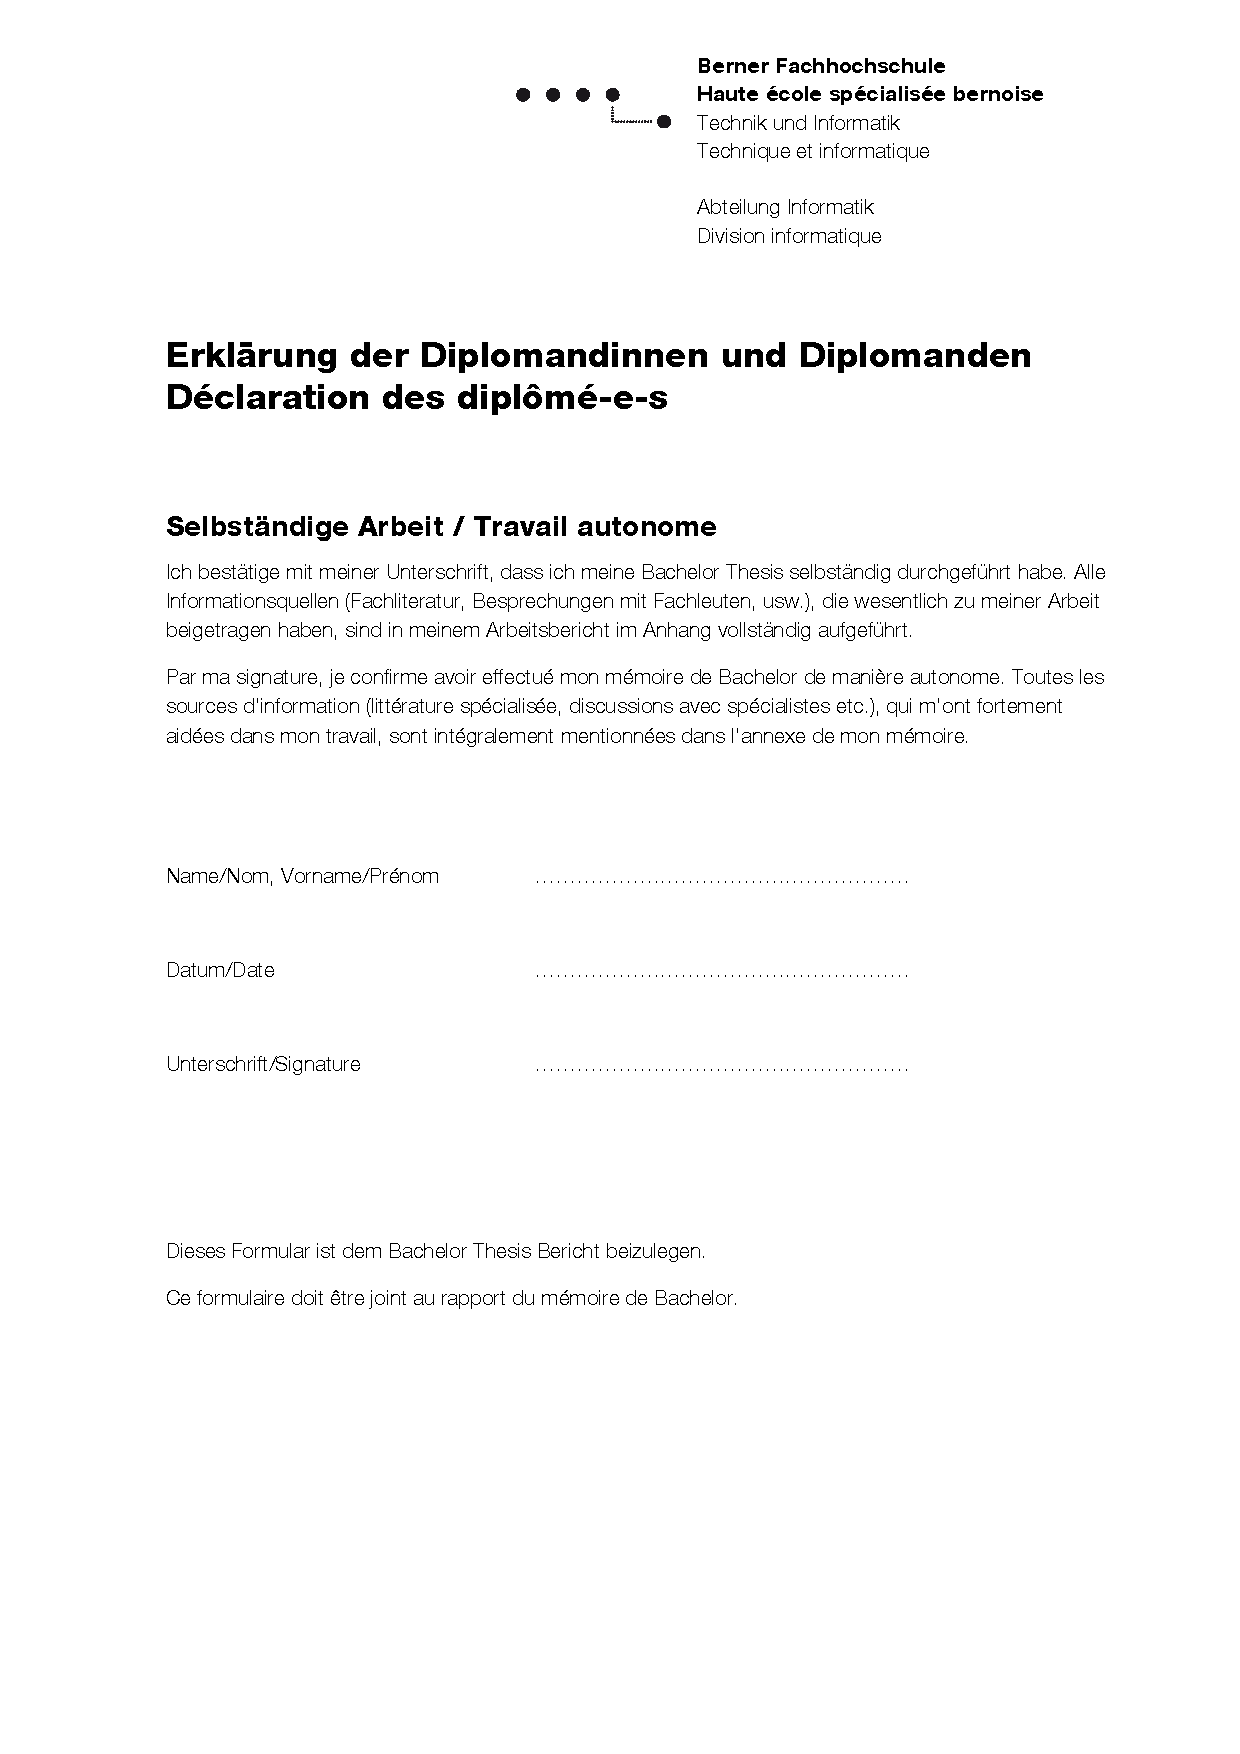
\includepdf{00_einleitung/Erklaerung.pdf}
\cleardoubleemptypage
\setcounter{page}{1}
\chapter*{Management Summary}
\label{chap:managementSummary}

Ants AI Challenge ist ein Programmierwettbewerb, bei welchem ein Bot programmiert wird der ein Ameisenvolk steuert. Das Ameisenvolk soll auf einer Map Futtersuchen sowie gegnerische V�lker angreifen und vernichten. Dabei m�ssen Problem wie die Pfadsuche, das Verteilen von Aufgaben sowie das Schwarmverhalten gel�st werden. In unserer Arbeit wollten wir herausfinden was es alles braucht um einen solchen intelligenten Bot zu schreiben und gegen andere Mitspieler anzutreten. Wir konzetrierten uns auf die Aufgabenverteilung sowie die Pfadsuche. Diese Erfahrungen wollen wir f�r die Bachelorarbeit mitnehmen, wo wir an einer aktiven Challenge teilnehmen m�chten oder uns in der f�r dieses Projekt verwendete Challenge vertiefen.

\vspace{5cm}
\begin{tabbing}
xxxxxxxxxxxxxxxxxxxx\=xxxxxxxxxxxxxxxxxxxxxxx \kill
Datum					\> \today \\ \\ \\
Name Vorname	\> Lukas Kuster \\ \\
Unterschrift	\> ......................................................... \\ \\ \\
Name Vorname	\> Stefan K�ser \\ \\
Unterschrift	\> .........................................................
\end{tabbing}


%---------------------------------------------------------------------------

% Table of contents and listings
%---------------------------------------------------------------------------
\tableofcontents
\listoffigures
\listoftables
\renewcommand*{\lstlistlistingname}{Listingsverzeichnis}
\lstlistoflistings
\cleardoublepage
%---------------------------------------------------------------------------
	
% Main part:
%---------------------------------------------------------------------------
\pagenumbering{arabic}

\chapter{Einleitung}
\label{chap:einleitung}
Nachdem wir uns im Rahmen des Moduls ''Projekt 2`` (7302) mit der Implementierung eines Bots f�r den Online-Wettbewerb Ants AI-Challenge\footnote{\url{http://www.aichallenge.org}} besch�ftigt hatten, haben wir uns f�r die Bachelorarbeit eine Verbesserung dieses Bots vorgenommen. Ziel des Wettbewerbs ist es jeweils, einen Bot zu programmieren, der durch geschickten Einsatz von KI-Technologien das Spiel m�glichst erfolgreich bestreiten kann.

Im ''Projekt 2`` hatten wir zwar einen Bot implementiert, der alle Aspekte des Spiels einigermassen beherrscht, dazu geh�ren Nahrung sammeln, die Gegend entdecken, H�gel erobern und verteidigen, sowie gegen feindliche Ameisen k�mpfen. Einige dieser F�higkeiten waren aber eher rudiment�r ausgebaut, da wir uns vor allem auf die Pfadsuche konzentriert hatten.

In der Bachelorarbeit ging es nun darum, die taktischen und strategischen Fertigkeiten des Bots auszubauen. Der Schwerpunkt lag auch bei der Bachelorarbeit nicht auf der Optimierung einer Teilaufgabe, sondern auf der Implementierung eines ausgewogenen Bots, der alle Aspekte des Spiels gleichermassen gut beherrscht.

Ein besonderes Augenmerk legten wir dabei auf einen modularen Aufbau des Codes. Nebst einem sauberen objektorientierten Programmdesign spiegelt sich das vor allem in den separaten Modulen ''AITools-Api``, ''Search`` und ''Strategy``, die so generisch implementiert wurden, dass sie mit geringem Aufwand auch in anderen Projekten einsetzbar sind.


%L DONE OK
\section{Spielbeschrieb}
\label{sec:einleitung.Spielbeschrieb}

\subsection{Der Wettbewerb}
\label{sec:einleitung.Spielbeschrieb.wettbewerb}
Die AI Challenge\footnote{\url{http://www.aichallenge.org}} ist ein internationaler Wettbwerb des University of Waterloo Computer Science Club der im Zeitraum Herbst 2011 bis Januar 2012 zum 3. Mal stattgefunden hat. Das Spiel in dieser 3. Ausf�hrung war ein zugbasiertes Multiplayerspiel in welchem sich Ameisenv�lker gegenseitig bek�mpfen. Ziel in der AI-Challenge ist es, einen Bot zu schreiben, der die gegebenen Aufgaben mit m�glichst intelligenten Algorithmen l�st. Die zu l�senden Aufgaben der Ants AI Challenge sind die Futtersuche, das Explorieren der Karten, das Angreifen von gegnerischen V�lkern und deren Ameisenhaufen sowie dem Sch�tzen des eigenen Ameisenhaufen.

\subsection{Spielregeln}
\label{sec:einleitung.Spielbeschrieb.spielregeln}
Nachfolgend sind die wichtigsten Regeln, die w�hrend dem Spiel ber�cksichtigt werden m�ssen, aufgelistet.
\begin{itemize} 
\item Pro Zug k�nnen alle Ameisen um ein Feld (vertikal oder horizontal) verschoben werden.
\item Pro Zug steht insgesamt eine Rechenzeit von einer Sekunde zur Verf�gung. Es d�rfen keine Threads erstellt werden.
\item Bewegt sich eine Ameise in die 4er Nachbarschaft eines Futterpixels, wird dieses eingesammelt. Beim n�chsten Zug entsteht bei einem Ameisenh�gel eine neue Ameise.
\item Die Landkarte besteht aus passierbaren Landpixeln sowie unpassierbaren Wasserstellen.
\item Ein Gegner wird geschlagen, wenn im Kampfradius der eigenen Ameise mehr eigene Ameisen stehen als gegnerische Ameisen im Kampfradius der Ameise, die angegriffen wird.
\item Ein Gegner ist ausgeschieden wenn alle seine eigenen Ameisenh�gel vom Gegner vernichtet wurden. Pro verlorenem H�gel gib es einen Punkteabzug. Pro feindlichen H�gel, der zerst�rt wird gibt es zwei Bonuspunkte.
\item Steht nach einer definierbaren Zeit (Anzahl Z�ge) kein Sieger fest, wird der Sieger anhand der Punkte ermittelt. 
\end{itemize}
Die ausf�hrlichen Regeln k�nnen auf der Webseite nachgelesen werden: \url{http://aichallenge.org/specification.php}

\subsection{Schnittstelle}
\label{sec:einleitung.Spielbeschrieb.schnittstelle}
Die Spielschnittstelle ist simpel gehalten. Nach jeder Spielrunde erh�lt der Bot das neue Spielfeld mittels String-InputStream, die Spielz�ge gibt der Bot dem Spielcontroller mittels String-OutputStream bekannt. Unser MyBot leitet von der Basis-Klasse Bot\footnote{Die Klasse ist im Code unter ants.bot.Bot.Java auffindbar } ab. Ein Spielzug wird im folgendem Format in den Output-Stream gelegt:
\newline
\newline
o <Zeile> <Spalte> <Richtung>
\newline
\newline
Beispiel:
\begin{verbatim}
o 4 7 W
\end{verbatim}
Die Ameise wird von der Position Zeile 4 und Spalte 7 nach Westen bewegt.
\newline
Der Spielcontroller ist in Python realisiert, der Bot kann aber in allen g�ngigen Programmiersprachen wie Java, Python, C\#, C++ etc. geschrieben werden.
 %DONE OK
\section{Abgrenzungen}
\label{sec:einleitung.Abgrenzungen}

Da unsere Arbeit auf dem vorg�ngigen Modul ''Projekt 2`` aufbaut, wurden nicht alle Module w�hrend der Bachelorarbeit erstellt. Wir haben im Modul ''Projekt 2`` auf einen sauberen Aufbau geachtet. So war es uns m�glich die meisten Komponenten zu �bernehmen. Es folgt eine Auflistung was bereits bestand bzw. was wir noch erweitert haben. Nicht aufgef�hrt sind w�hrend der Bachelorarbeit komplett neu hinzugekommene Funktionalit�ten wie die \gls{InfluenceMap} oder die Profile.

\renewcommand{\arraystretch}{1.5}
\begin{table}[H]
	\centering
 \begin{tabular}{l p{10cm}}
  \textbf{Erstellt in Modul ''Projekt 2``} & \textbf{Erweiterung w�hrend der Bachelorarbeit} \\
	\hline
  Grundfunktionalit�ten des Bots & --\\ 
  Pfadsuche Simple, A*, HPA*  & Auslagerung in ein eigenes Framework, Performanceverbesserungen, Erweiterung des HPA* Clustering, Pfadsuche unter Ber�cksichtigung der \gls{InfluenceMap}, Breitensuche\\
  Logging											& Loggen in verschiedene Logfiles, \gls{LazyInitialization} \\
  Tasks 		& Die Funktionsweise jedes Tasks wurden nochmals �berdacht und angepasst\\
  Missionen & Die Missionen wurden verfeinert und mit strategischen und taktischen Entscheidungen erweitert \\
  \gls{MinMaxAlgorithmus} & Bei den Kampfsituationen wurde versucht, den MinMax Algorithmus einzubauen, welchen wir bereits im Modul Spieltheorie erarbeitet hatten. (Mehr dazu siehe Kapitel \ref{sec:module.MinMax}) \\
 \end{tabular}
\caption{Abgrenzungen}
\end{table}
%S DONE OK OK
\section{Projektverlauf}
\label{sec:einleitung.Projektverlauf}

Die Projektarbeit richtete sich nach folgendem Zeitplan:

\begin{figure}[bth]
\centering
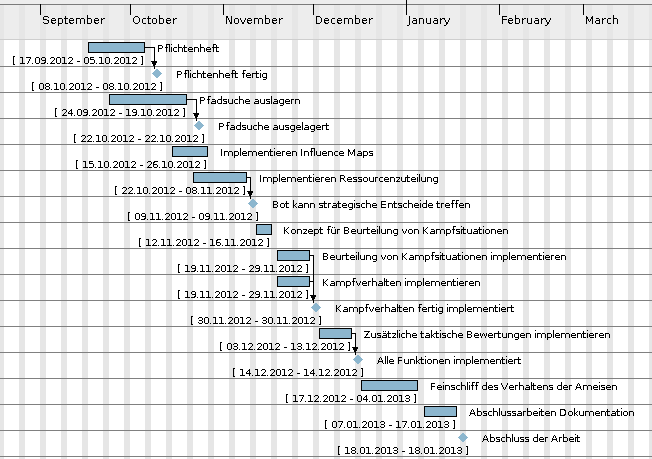
\includegraphics[width=0.9\textwidth]{91_bilder/gantt}
\caption{Projektablauf}
\label{fig:gantt}
\end{figure}
% \begin{tabular}{p{3cm}l}
%   \hline
%  \textbf{Datum} 			& \textbf{Arbeit}   \\
%  \hline
%  17.09.2012 	& Start der Arbeit \\
%  06.10.2012 	& Fertigstellung des Pflichtenhefts \\
%  19.10.2012 	& Framework zur Pfadsuche fertiggestellt \\
%  09.11.2012	& Bot kann strategische Entscheide treffen \\
%  16.11.2012	& Konzept f�r die Bewertung der Kampfformationen \\
%  30.11.2012	& Kampfverhalten implementiert \\
%  15.12.2012	& Programmierung gr�ssten Teils abgeschlossen \\
%  15-31.12.2012 & Korrekturen \& Feinschliff des Bots \\
%  11.01.2013	& Fertigstellung der Arbeit \\
%  11-18.01.2013		& Reserve \\
%  18.01.2013 	& Abgabe der Arbeit \\
%  tbd				 	& Verteidigung Bachelor Arbeit \\ 
% \end{tabular} %L DONE OK
\section{Projektorganisation}
\label{sec:einleitung.Projektorganisation}

\subsection{Beteiligte Personen}
\label{sec:einleitung.Projektorganisation.BetroffenePersonen}

\textbf{Studierende:}\\
 Lukas Kuster \textit{kustl1@bfh.ch} \\
 Stefan K�ser \textit{kases1@bfh.ch}
 
\textbf{Betreuung:}\\
Dr. J�rgen Eckerle \textit{juergen.eckerle@bfh.ch}

\textbf{Experte:}\\
Dr. Federico Fl�ckiger	\textit{federico.flueckiger@bluewin.ch}


\subsection{Projektmeetings}
\label{sec:einleitung.Projektorganisation.Projektmeetings}

\begin{itemize}
\item Es fand jeweils ein Treffen mit dem Betreuer alle 1-2 Wochen statt.
\item Ein Treffen mit dem Experten fand am Anfang der Arbeit statt. Ein zweites Meeting wurde von beiden Seiten nicht f�r notwendig erachtet.
\end{itemize}

\subsection{Arbeitsweise}
\label{sec:einleitung.Projektorganisation.Arbeitsweise}

F�r die gemeinsame Arbeit am Projekt hatten wir uns jeweils den Freitag reserviert. An diesen Tagen arbeiteten wir meist mit Pair-Programming und erzielten dabei gute Fortschritte. Die verbleibenden Aufgaben teilten wir uns auf und arbeiteten einzeln daran. Dabei war die Versionskontrolle mit Git ein sehr hilfreiches Tool, um die Arbeiten zu koordinieren.

Wir arbeiteten mit einem zentralen, �ffentlichen Repository auf GitHub (\url{https://github.com/koschder/ants/}). Nebst dem Vorteil einer vereinfachten Zusammenarbeit bietet GitHub auch einige graphische Auswertungen der Aktivit�t in einem Projekt, die Aufschluss �ber den Verlauf unserer Arbeit geben.

\begin{figure}[H]
\centering
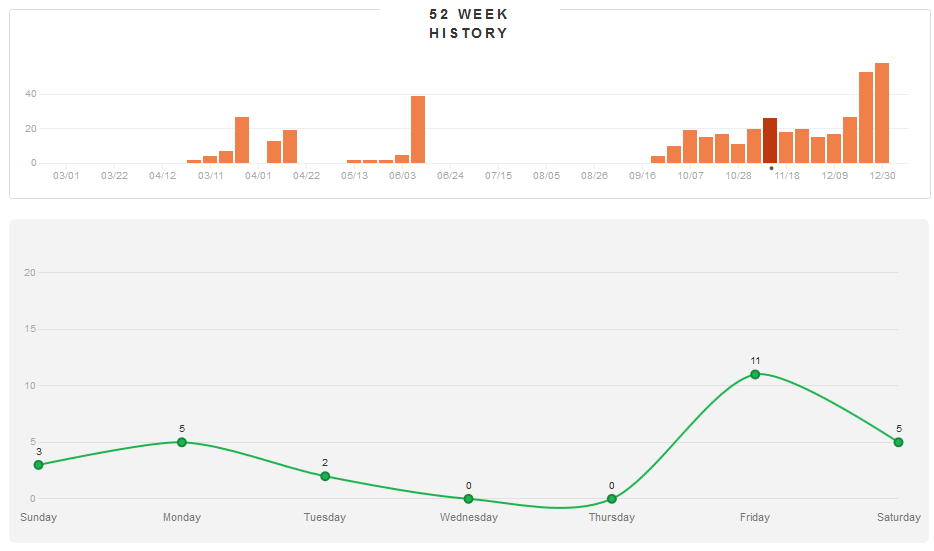
\includegraphics[width=0.99\textwidth]{91_bilder/github/commits}
\caption{Commit History}
\label{fig:commits}
\end{figure}

Die obere H�lfte der Abbildung \ref{fig:commits} zeigt den Aktivit�tsverlauf des Projekts r�ckblickend auf das letzte Jahr. Links, w�hrend den Monaten M�rz, April, Mai und Juni ist der Verlauf des Projekts 2 zu sehen, nach der Sommerpause der Verlauf der Bachelorarbeit. Die Aktivit�tssteigerung gegen Ende des Projekts ist vor allem auf Dokumentations- und Aufr�umarbeiten zur�ckzuf�hren.

Die untere H�lfte zeigt die Anzahl Commits �ber eine Woche verteilt. Man sieht sch�n, dass der Freitag mit Abstand der produktivste Tag war, mit reduzierter Aktivit�t �ber den Rest der Woche verstreut.

\begin{figure}[H]
\centering
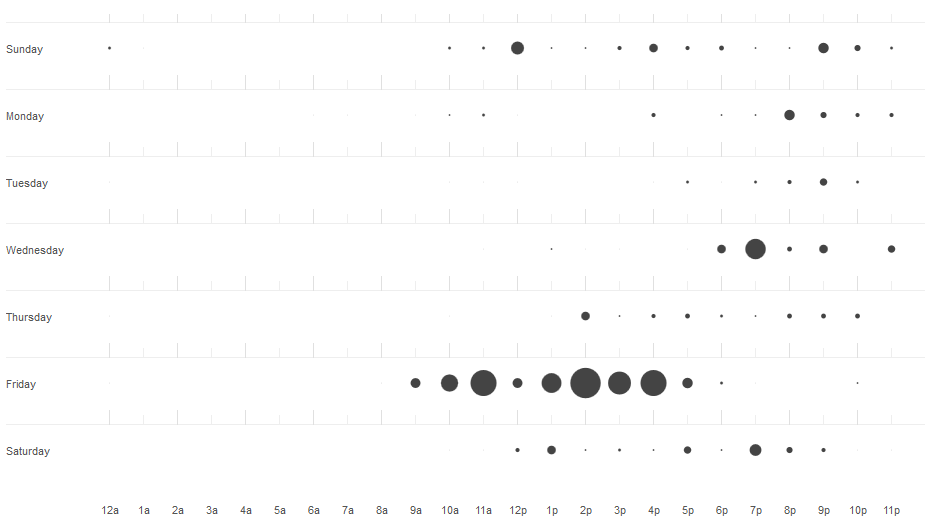
\includegraphics[width=0.99\textwidth]{91_bilder/github/punchcard}
\caption{Aktivit�ten}
\label{fig:punchcard}
\end{figure}

Abbildung \ref{fig:punchcard} zeigt f�r den gesamten Projektverlauf die Zeiten mit der gr�ssten Aktivit�t. Auch hier kann man deutlich erkennen, dass der gr�sste Teil der Arbeit an den Freitagen erstellt wurde.

%L DONE OK
\section{Tools}
\label{sec:einleitung.Tools}

F�r diese Arbeit verwendeten wir folgende Tools:
\begin{itemize}
\item Eclipse f�r die Java-Entwicklung (\url{http://www.eclipse.org})
\item ANT f�r die Build-Automatisierung (\url{http://ant.apache.org})
\item Git (\url{http://git-scm.com}) f�r die Versionskontrolle, mit einem zentralen Repository f�r die einfachere Zusammenarbeit auf GitHub (\url{http://www.github.com})
\item TeXnicCenter (\url{http://www.texniccenter.org}) und MiKTeX (\url{http://miktex.org}) f�r die Dokumentation in \LaTeX
\item GanttProject (\url{http://www.ganttproject.biz}) f�r den Zeitplan
\item Visual Paradigm for UML (\url{http://www.visual-paradigm.com/product/vpuml/}) f�r die UML-Diagramme
\end{itemize}%L DONE OK
\section{Artefakte}
\label{sec:einleitung.Artefakte}

Folgende Artefakte werden zusammen mit dieser Dokumentation in elektronischer Form abgegeben:
\begin{itemize}
\item Der komplette Source-Code inklusive Git-History
\item Ein Archiv mit der generierten Code-Dokumentation (Javadoc)
\item Ein Archiv mit den Testprotokollen
\item Das Pflichtenheft
\end{itemize}
%L DONE OK

\newcommand{\vspacecm}{0.7cm}

\chapter{Ziele}

Der im Rahmen von Projekt 2 entwickelte Bot soll um Logik f�r taktische und strategische Entscheidungen und koordinierte Bewegung erweitert werden.

\section{Funktionale Anforderungen}
\label{sec:ziele.FunktionaleAnforderungen}

\subsection{Musskriterien}
\label{sec:ziele.FunktionaleAnforderungen.Musskriterien}

Der Bot unterscheidet zwischen diversen Aufgaben:
	\begin{itemize}
	\item Nahrungsbeschaffung
	\item Angriff
	\item Verteidigung
	\item Erkundung
	\end{itemize}

\vspace{\vspacecm}

Der Bot kann eine Beurteilung seiner Situation auf dem Spielfeld vornehmen
	\begin{itemize}
	\item Dominante/unterlegene Position
	\item Sicherheit verschiedener Gebiete des Spielfelds (eigener/gegnerischer Einfluss)
	\item Konfliktpotenzial in verschiedenen Gebieten des Spielfelds
	\end{itemize}
		
Anhand der Situationsbeurteilung werden die unterschiedlichen Aufgaben entsprechend gewichtet. Stark gewichtete Aufgaben erhalten mehr Ressourcen (Ameisen) zur Durchf�hrung.

\vspace{\vspacecm}

Der Bot identifiziert zur Erf�llung dieser Aufgaben taktische Ziele:
	\begin{itemize}
	\item Gegnerische H�gel angreifen, was bei Erfolg den Score erh�ht und das eigentliche Ziel des Spiels ist.
	\item Isolierte gegnerische Ameisen angreifen.
	\item Schwachstellen in der gegnerischen Verteidigung ausnutzen.
	\item Engp�sse im Terrain sichern bzw. versperren.
	\item Konfliktzonen, d.h. viele Ameisen auf einem engen Raum, erkennen und entsprechend reagieren.
	\end{itemize}

\vspace{\vspacecm}

F�r die konkrete Erreichung dieser definierten Ziele verf�gt der Bot �ber taktische Logik:
	\begin{itemize}
	\item Bei der Pfadsuche wird die Sicherheit der zu durchquerenden Gebiete ber�cksichtigt
	\item In Kampfsituationen kann der Bot die Ameisen in Formationen gliedern, die geeignet sind, eine lokale �berzahl eigener gegen�ber gegnerischen Ameisen zu erzeugen
	\item Beim Aufeinandertreffen mit gegnerischen Ameisen wird Entschieden ob angegriffen, die Stellung gehalten oder gefl�chtet wird.
	\end{itemize}

\subsection{Kannkriterien}
\label{sec:ziele.FunktionaleAnforderungen.Kannkriterien}
Das Verhalten des Bots ist konfigurativ einstellbar, so dass zum Beispiel ein �agressiver� Bot gegen einen defensiven Bot antreten kann.

\section{Nicht funktionale Anforderungen}
\label{sec:ziele.NichtFunktionaleAnforderungen}

\subsection{Musskriterien}
\label{sec:ziele.NichtFunktionaleAnforderungen.Musskriterien}
Modularer Aufbau, so dass die einzelnen Komponenten getestet werden k�nnen.

Wichtige Funktionen wie die Pfadsuche und die Berechnung von Influence Maps sollen in separaten Modulen implementiert werden, damit sie auch von anderen Projekten verwendet werden k�nnten.

Der Code wird dokumentiert, so dass dieser nachvollziehbar ist.

\subsection{Kannkriterien}
\label{sec:ziele.NichtFunktionaleAnforderungen.Kannkriterien}
F�r die wiederverwendbaren Module wird jeweils ein kleines Tutorial geschrieben, wie die Module verwendbar sind.


\section{Abgrenzungskriterien}

TODO%L DONE OK
\section{Herausforderungen}
\label{sec:einleitung.Herausforderungen}

\subsection{Module testen}
\label{sec:einleitung.Herausforderungen.ModuleTesten}

Ein neuer Algorithmus oder eine neue Idee ist schnell mal in den Bot integriert, doch bringen die geschriebenen Zeilen den gew�nschten Erfolg? Was wenn der neue Codeabschnitt �usserst selten durchlaufen wird und dann noch fehlschl�gt? Wie wissen wir welche Ameise genau diesen n�chsten Schritt macht?
\newline
\newline
Um diese Probleme zu bew�litgen haben wir ein ausgekl�geltes Logging auf die Beine gestellt, in welchem wir schnell an die gew�nschten Informationen gelangen. (siehe \ref{sec:module.Logging})  Zudem k�nnen wir dank der Erweiterung des HTML-Viewer sofort sehen, welches die akutelle Aufgabe jeder einzelen Ameise ist. (siehe \ref{sec:module.Logging.Addon}) Weitergeholfen haben uns auch etliche Unit- und Funktionstests, mit welchen wir neu geschriebenen Code testen und auf dessen Richtigkeit pr�fen konnten. (siehe \ref{sec:testCenter.UnitundFunktionstests})

\subsection{TODO}
\label{sec:einleitung.Herausforderungen.TODO}
lorem ipsum mehr herausfoderungen ??

\subsection{Vergleich mit Bots aus dem Wettbewerb}
\label{sec:einleitung.Herausforderungen.VergleichBots}
Nach Ablauf des Wettbewerbs im Januar 2012, haben einige der Teilnehmer ihren Bot zug�nglich gemacht. Dadurch war es uns m�glich unseren Bot gegen Bots antreten zu lassen die tats�chlich am Wettbewerb teilgenommen haben. So konnten wir auch eine wage Einsch�tzung machen wir stark unser Bot ist. Mehr dazu unter siehe \ref{sec:testCenter.TestreportProfile}.%L DONE OK
\section{Weiterf�hrende Arbeiten}
\label{sec:einleitung.Weiterf�hrendeArbeiten}

M�gliche weiterf�hrende Arbeiten sind...

- mehr Regeln f�r Ressourcenverwaltung
- Profile erweitern
- raffinierteres CombatPositioning%L DONE OK
\section{Fazit}
\label{sec:einleitung.Fazit}
Alles in allem sind wir mit dem Verlauf der Arbeit zufrieden. Wir konnten unsere Ziele erreichen und konnten dank einer strukturierten Arbeitsweise auch den Zeitplan gr�sstenteils einhalten. 
In Bezug auf die Wettbewerbsf�higkeit des Bots hatten wir uns bewusst keine konkreten Ziele gesetzt, da wir wussten, dass es in der beschr�nkten Zeit sehr schwierig werden w�rde, mit den Top 100 des Wettbewerbs mitzuhalten. Insofern sind wir auch mit dem Ergebnis zufrieden: Gegen den Bot (\gls{Egreavette}) mit Schlussrang 93 konnten wir rund 60\% der Spiele gewinnen, und gegen den Sieger des Wettbewerbs (\gls{xathis})  immerhin um die 20\% der Spiele. (Details s. Kapitel \ref{sec:testCenter.TestreportProfile})

Besonders positiv hervorheben m�chten wir die Arbeitsprozesse und Tools, die uns diesen guten Projektverlauf erm�glicht haben. Die w�chentlichen Treffen mit \gls{PairProgramming} waren dabei besonders produktiv; unter der Woche konnten wir uns dank einer guten Arbeitsaufteilung und der Unterst�tzung durch die Versionsverwaltung jeweils auf das Wesentliche konzentrieren, ohne durch administrative oder technische Probleme abgelenkt zu werden.

Ausserdem war nat�rlich die Arbeit am Bot sehr spannend, da wir hier die Gelegenheit hatten, den in den letzten 8 (und insbesondere den letzten 3) Semestern behandelten Stoff in die Praxis umzusetzen. Besonders interessant war dabei die Herausforderung, die einzelnen, isolierten Techniken, die wir gelernt hatten, zu einem strukturierten Ganzen zusammenzuf�gen.

Ein kleiner Wermutstropfen bleibt nat�rlich, dass wir unseren Bot nicht unter Wettbewerbsbedingungen testen konnten; die Testl�ufe gegen die verschiedenen Gegner erlaubten uns zwar eine ungef�hre Standortbestimmung, aber das ist nat�rliche nicht das Gleiche. Auch sind wir, wie bereits erw�hnt, nicht ganz zufrieden mit der Implementierung des Kampfverhaltens unserer Ameisen. Mit etwas mehr Zeit h�tten wir da gerne noch eine genauere und dynamischere Bewertung von Kampfsituationen eingebaut.%L DONE OK
\section{Anmerkungen zur Dokumentation}
\label{sec:einleitung.Anmerkungen}
Hier noch einige Anmerkungen zur Dokumentation:

\paragraph{Diagramme}
S�mtliche \gls{UML}-Diagramme stellen jeweils eine vereinfachte Sicht dar und erheben keinen Anspruch auf Vollst�ndigkeit. Bei den Diagrammen, die einzelne Packages darstellen, sind jeweils Klassen oder Interfaces, die eigentlich aus einem anderen Package stammen, farblich hervorgehoben.

\paragraph{Listings}
Die meisten Listings sind zwar direkt aus dem Code unseres Bots kopiert. Der Lesbarkeit halber wurden sie jedoch mehr oder weniger stark gek�rzt und einzelne Abschnitte wurden durch Pseudocode ersetzt.%L DONE OK

\chapter{Architektur}
\label{chap:Architektur}

\section{Module}
\label{sec:architektur.Module}

\begin{figure}[H]
\centering
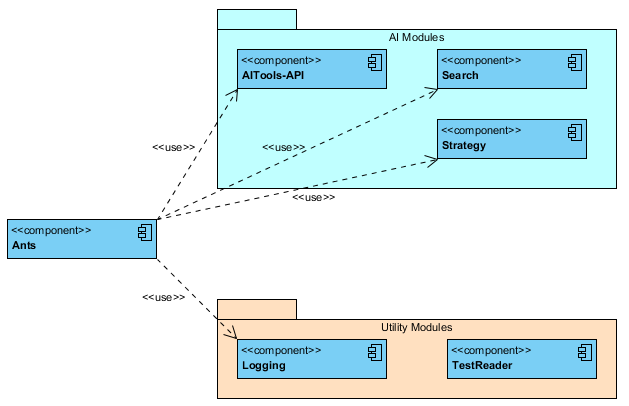
\includegraphics[width=0.9\textwidth]{91_bilder/modulesOverview}
\caption{Module}
\label{fig:modulesOverview}
\end{figure}

Abbildung \ref{fig:modulesOverview} zeigt die Gliederung des Bots in die verschiedenene Untermodule. Wir unterscheiden dabei zwischen den AI Modulen, welche die eigentliche AI-Logik enthalten, und den Utility Modulen, die Basisfunktionen wie Logging implementieren.

\paragraph{Ants:} Das Ants Modul enth�lt das Grundger�st des Bots und f�gt die anderen Module zu einem Ganzen zusammen. Es ist das einzige Modul, in dem Ants-spezifische Funktionalit�ten implementiert sind; die anderen sind generisch gehalten um die Wiederverwendbarkeit sicherzustellen.

\paragraph{AITools-API:} Im API-Modul sind alle gemeinsamen Interfaces definiert, auf die die anderen Module zugreifen. Zum Teil ist hier auch Basis-Funktionalit�t implementiert, wie z.B. Distanzberechnungen auf einer Karte.

\paragraph{Search:} Dieses Modul enth�lt unsere Implementationen zur Pfad- und Breitensuche.

\paragraph{Strategy:} Das Strategy-Module enth�lt strategische und taktische Algorithmen, insbesondere die Influence Map und das CombatPositioning.

\paragraph{Logging:} Das Logging-Modul definiert ein flexibles Logging-Framework.

\paragraph{TestReader:} Das TestReader-Modul besteht aus einer einzelnen Klasse, die aus den Log-Files der Ants-Spielengine Auswertungen lesen kann.

\section{Modulabh�ngigkeiten}
\label{sec:architektur.Modulabh�ngigkeiten}


\begin{figure}[H]
\centering
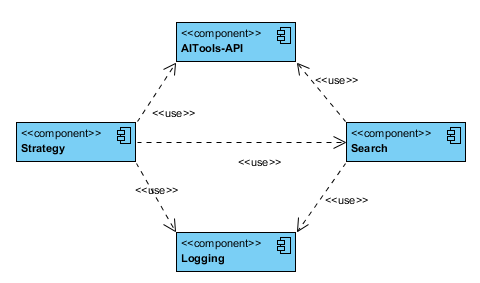
\includegraphics[width=0.8\textwidth]{91_bilder/modulesDependencies}
\caption{Modulabh�ngigkeiten}
\label{fig:modulesDependencies}
\end{figure}
Abbildung \ref{fig:modulesDependencies} zeigt die Abh�ngikeiten zwischen den Modulen. Die Module API und Logging sind unabh�ngig, w�hrend die beiden gr�sseren Module Abh�ngigkeiten auf API und Logging haben.
Die Abh�ngigkeit von Strategy auf Search r�hrt daher, dass die Influence Map mittels FloodFil Algorithmus aufgebaut wird, der im Search Modul implementiert ist.

\section{Externe Abh�ngigkeiten}
\label{sec:architektur.externeAbh�ngigkeiten}
Der Bot selber (also der Code, der von der Spielengine aufgerufen wird) hat keine externen Abh�ngigkeiten - dies w�re von den Regeln des Wettbewerbs auch gar nicht erlaubt gewesen. F�r ein paar andere Zwecke haben wir aber trotzdem auf externe Programmbibliotheken zur�ckgegriffen.

\begin{itemize}
\item
\textbf{JUnit \url{http://junit.org}:} F�r unsere zahlreichen Unit- und Funktions-Tests verwendeten wir Junit.
\item
\textbf{ClasspathSuite \url{http://johanneslink.net/projects/cpsuite.jsp}:} Da JUnit keine bequemen Weg bietet, alle Tests aus verschiedenen Projekten auf einmal auszuf�hren, verwendeten wir die ClasspathSuite, um die Tests direkt in Eclipse auszuf�hren.
\item
\textbf{Json-simple \url{http://code.google.com/p/json-simple/}:} Json-simple ist eine einfache Json-Parsing Bibliothek, die wir im TestReader verwenden, um die Json-Logs der Spielengine auszuwerten.
\end{itemize}%L DONE OK

\chapter{API}
\label{sec:module.API}

Unsere AITools API dient als Grundbaustein des gesamten Projekt. Sie entkapselt die Interfaces zu unseren Search- und Strategieimpelementierungen. Sie beinhaltet zudem Basisklassen, welche �berall verwendet werden. Der Inhalt ist wie folgt:

\section{Entities}
\label{sec:mocule.API.Entities}

\begin{figure}[H]
\centering
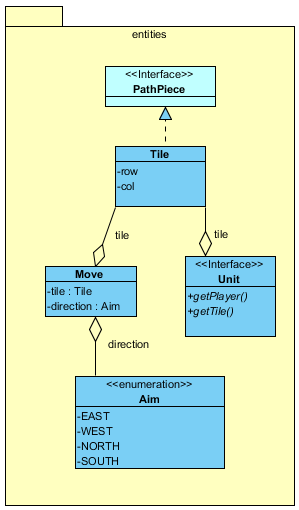
\includegraphics[width=0.5\textwidth]{91_bilder/apiEntities}
\caption{Entities}
\label{fig:apiEntities}
\end{figure}

\begin{itemize}
\item
\textbf{Aim}: Richtungangabe zum Beschreiben einer Bewegung der Ameise
\item
\textbf{Tile}: Repr�sentiert eine Zelle auf dem Spielfeld, welche mit Row (Zeile) und Column (Spalte) beschrieben ist.
\item
\textbf{Move}: Diese Klasse beschreibt einen Spielzug mit den Eigenschaften Tile, von wo aus der Zug statt findet, und Aim, in welche Richtung der Zug ausgef�hrt wird.
\item
\textbf{Unit}: Unit besteht aus Tile und Spieler und definiert eine Einheit eines Spielers auf der Karte.
\end{itemize}

\section{Map}
\label{sec:mocule.API.Map}

\begin{figure}[H]
\centering
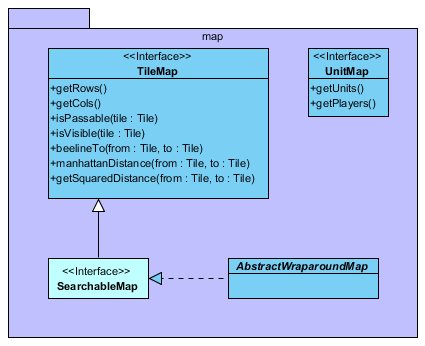
\includegraphics[width=0.7\textwidth]{91_bilder/apiMap}
\caption{Map API}
\label{fig:apiMap}
\end{figure}

\begin{itemize}
\item
\textbf{TileMap}:  Dieses Interface definiert, welche Methoden eine auf Tiles aufbauende Spielkarte anbieten muss. Dazu geh�ren die Masse der Karte, ob ein Tile auf der Karte sichtbar und passierbar ist, sowie Distanz Messfunktion wie ManhattanDistanz, Luftlinie, quadrierte Distanz.
\item
\textbf{UnitMap}: UnitMap ist auch ein Interface welches auf TileMap aufbaut und zus�tzlich die Methoden definiert die Einheiten und Spieler zur�ckzugeben.
\item
\textbf{AbstractWraparoundMap}: Implementiert das Interface SearchableUnitMap (siehe: Abschnitt Search). Hier sind alle Methoden implementiert, welche die Karte anbieten muss, damit sie mit den Suchalgorihmen verwendet werden kann. Zudem sind die Methoden aus TileMap implementiert. Diese geben �ber die Gel�ndebeschaffenheit und Distanzen Auskunft.
\item
\textbf{WorldType}: WorldType ist ein Enum und definiert die Art der Karte. Der Typ Globus hat keine Kartenr�nder, ist also ringsum begehbar. Von diesem Typ ist auch die Ants Challenge somit auch die Klasse AbstractWraparoundMap. Der zweite Enumtyp ist Pizza und definiert eine Welt so wie unsere Erde vor 500 Jahren noch definiert wurde, eine Scheibe mit R�ndern, welche die Welt begrenzen. Dieser zweite Typ wurde provisorisch erstellt. Falls diese API eine Weiterverwendung findet, kann dieser Typ zus�tzlich implementiert werden.
\end{itemize}


\section{Search}
\label{sec:mocule.API.Search}

\begin{figure}[H]
\centering
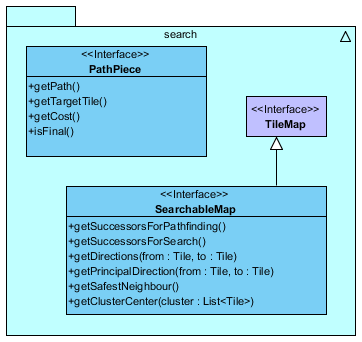
\includegraphics[width=0.6\textwidth]{91_bilder/apiSearch}
\caption{Search API}
\label{fig:apiSearch}
\end{figure}

\begin{itemize}
\item
\textbf{PathPiece}: Das PathPiece ist ein Interface f�r Strukturen, die als Suchknoten in der Pfadsuche verwendet werden k�nnen. Es definiert die f�r die Suche n�tigen Methoden, wie getSuccessors(), getCost(), oder getPath(). 
Implementierende Klassen sind Edge (rep�sentiert eine Kante in einem Cluster) und Tile. Erweiterungen dieser Klassen sind DirectedEdge (eine gerichtete Kante) und Vertex (eine Zelle mit zugeh�rigen Kanten).
\item
\textbf{SearchableMap}: Das Interface SearchableMap erweitert das Interface TileMap. Es beschreibt die Methoden zur Pfadsuche.
\item
\textbf{SearchableUnitMap}: Dieses Interface dient ausschliesslich zur Zusammenf�hrung der beiden Interfaces UnitMap und SearchableMap.
\end{itemize}

\section{Strategy}
\label{sec:mocule.API.Strategy}

\begin{figure}[H]
\centering
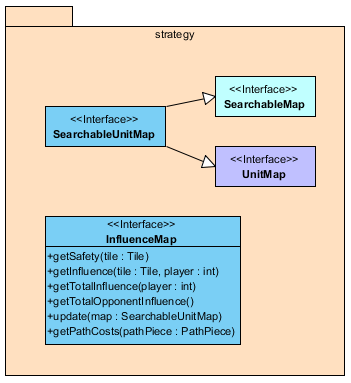
\includegraphics[width=0.6\textwidth]{91_bilder/apiStrategy}
\caption{Strategy API}
\label{fig:apiStrategy}
\end{figure}%S DONE OK
\chapter{Suchalgorithmen}
\label{sec:module.Suchalgorithmen}

\section{Enities f�r die Pfadsuche}
\label{sec:module.Suchalgorithmen.Enities}

\begin{figure}[H]
\centering
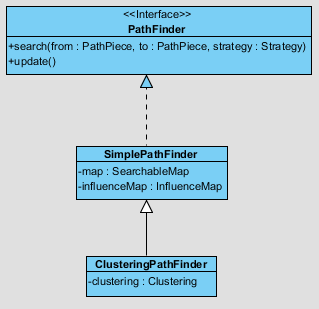
\includegraphics[width=0.6\textwidth]{91_bilder/pathfinderPathfinder}
\caption{Klassendiagramm Pfadsuche}
\label{fig:pathfinderPathfinder}
\end{figure}

\begin{figure}[H]
\centering
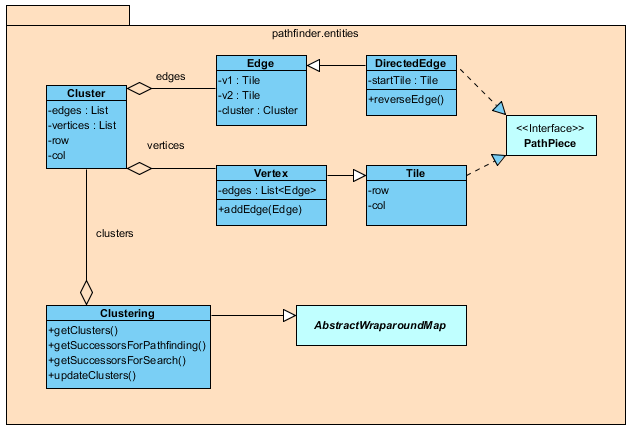
\includegraphics[width=0.9\textwidth]{91_bilder/pathfinderEntities}
\caption{Spiel-Elemente f�r die Suche (vereinfacht)}
\label{fig:pathfinderEntities}
\end{figure}


TODO NEW IMAGE

Abbildung \ref{fig:pathfinderEntities} zeigt die wichtigsten Klassen, die f�r die Pfadsuche verwendet werden. Der \"Ubersichtlichkeit wegen wurden nur die wichtigsten Attribute und Operationen in das Diagramm aufgenommen.

\section{Pfadsuche}
\label{sec:module.Suchalgorithmen.Pfadsuche}
Wir haben drei m�gliche Pfadalgorithmen in unserem Code eingebaut. Via PathFinder-Klasse kann f�r die Pfadsuche der Algorithmus ausgew�hlt werden.

\begin{figure}[H]
\centering
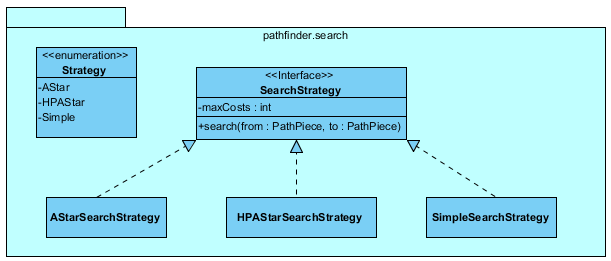
\includegraphics[width=0.9\textwidth]{91_bilder/pathfinderSearch}
\caption{Suchstrategien}
\label{fig:pathfinderSearch}
\end{figure}

\subsection{Simple Algorithmus}
\label{subsec:module.Suchalgorithmen.Pfadsuche.Simple}

Der Simple Algorithmus versucht das Ziel zu erreichen indem er zuerst die eine, dann die andere Achse abl�uft. Sobald ein Hindernis in den Weg kommt, bricht der Algorithmus ab. In der Abbildung \ref{fig:SimplePath} sucht der Algorithmus zuerst den Vertikal-Horizontal Pfad. Da dieser Pfad wegen dem Wasserhindernis (blau) nicht ans Ziel f�hrt, wird via Horizontal-Vertikal Pfad gesucht. Hier wird ein Pfad gefunden. Dieser Algorithmus ist, wie der Name bereits aussagt, sehr einfach aufgebaut und kostet wenig Rechenzeit. Daf�r kann er keinen Hindernissen ausweichen.

\begin{figure}[H]
\centering

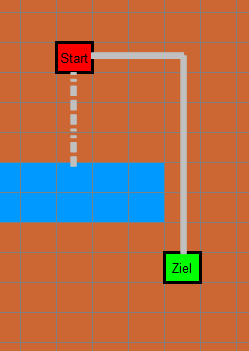
\includegraphics[height=50mm]{91_bilder/simplepath}
\caption{Simple-Path Algorithmus}
\label{fig:SimplePath}
\end{figure}

Folgendes Codesnippet zeigt auf wie ein Pfad mittels Pfadsuche Simple gefunden wird. Ein SimplePathFinder wird mit der Karte initialisiert. Danach kann die Suche mit pf.search(...) gestartet werden. Als Parameter wird der Suchalgorithmus Strategy.Simple, der Startpunkt (Position der Ameise) und Endpunkt (Position des Futters), sowie die maximalen Pfadkosten (hier: 16) mitgegeben.

\lstset{language=Java, tabsize=4}
\begin{lstlisting}
SimplePathFinder pf = new SimplePathFinder(map);
List<Tile> path = pf.search(PathFinder.Strategy.Simple, ant.getTile(), foodTile,16);
\end{lstlisting}

\subsection{A* Algorithmus}
\label{subsec:module.Suchalgorithmen.Pfadsuche.Astar}
Beim A* Algorithmus werden f�r jeden expandierten Knoten die gesch�tzten Kosten f(x) f�r die gesamte Pfadl�nge berechnet. f(x) besteht aus einem Teil g(x) welches die effektiven Kosten vom Startknoten zum aktuellen Knoten berechnet. Der andere Teil h(x) ist ein heuristischer Wert, der die Pfadkosten bis zum Zielknoten approximiert. Dieser Wert muss die effektiven Kosten zum Ziel immer untersch�tzen. Dies ist in unserem Spiel dadurch gegeben, dass sich die Ameisen nicht diagonal bewegen k�nnen, wir aber f�r den heuristischen Wert die Luftlinie zum Ziel verwenden. Die Pfadsuche wird immer bei dem Knoten fortgesetzt welcher die kleinsten Kosten f(x) hat.

Die Abbildung \ref{fig:heuristicAstar} zeigt den effektiven Pfad (grau) vom zu expandierenden roten Knoten mit den minimalen Kosten von 10 Pixel. Die Luftlinie (blau) als heuristischer Wert hat aber nur eine L�nge von 7.6 Pixel. Damit erf�llt unsere Heuristik die Anforderungen des Algorithmus.

Eine Pfadsuche mit A* wird gleich ausgel�st wie die Suche mit dem Simple-Algorithmus, ausser dass als Parameter die Strategy AStar gew�hlt wird.

\lstset{language=Java, tabsize=4}
\begin{lstlisting}
SimplePathFinder pf = new SimplePathFinder(map);
List<Tile> path = pf.search(PathFinder.Strategy.AStar, ant.getTile(), foodTile,16);
\end{lstlisting}

\begin{figure}[H]
\centering
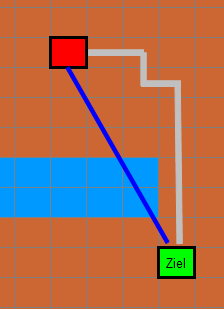
\includegraphics[height=50mm]{91_bilder/heuristicAstar.png}
\caption[A* Pfadsuche]{Heuristische Kosten (blau), Effektive Kosten (grau)}
\label{fig:heuristicAstar}
\end{figure}

Dieser A*-Algorithmus wird in unserem Code f�r eine Pfadsuche �ber alle Pixel (jedes Pixel ist ein Node) verwendet. Der gleiche Code wir aber auch f�r die Pfadsuche mit dem Pfadnetz des HPA* verwendet.

\subsection{HPA* Algorthmus}
\label{subsec:module.Suchalgorithmen.Pfadsuche.HPAstar}

Eine Pfadsuche A* �ber alle Pixel ist sehr teuer, da es viel Pfade gibt, die zum Teil nur ein Pixel nebeneinander liegen. Es werden bis zum Schluss verschiedenen Pfaden nachgegangen. Abhilfe zu dieser sehr feinmaschigen Pfadsuche bietet der Hierarchical Pathfinding A* bei welchem im sogenannten Clustering �ber mehrere Pixel verlaufende Kanten und Knoten berechnet werden.

\subsubsection{Clustering}
Das Clustering wird w�hrend dem ClusteringTask ausgef�hrt, Dabei wird die Landkarte in sogenannte Clusters unterteilt. Auf dem Bild \ref{fig.clusteredMap} wurde die Karte in 16 Clusters aufgeteilt.

\begin{figure}[H]
\centering
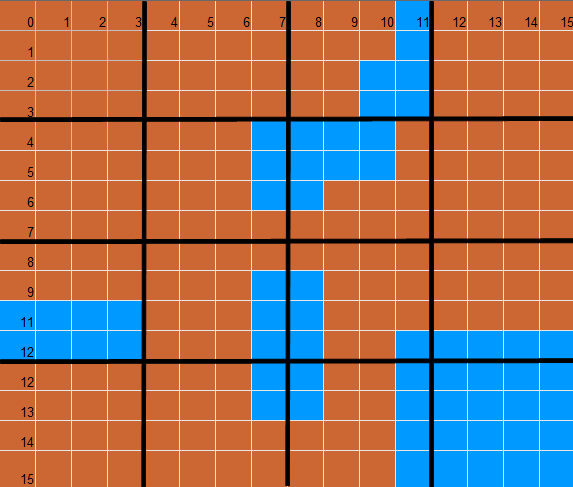
\includegraphics[height=50mm]{91_bilder/clusteredMap.png}
\caption[Clustereinteilung auf der Landkarte.]{Clustereinteilung auf der Landkarte. Clustergr�sse 4x4, Landkarte 16x16}
\label{fig.clusteredMap}
\end{figure}

Wir unterschieden zwischen den zwei Clusterarten Centered und Corner. Die Variante Corner wurde bereits im Vormodule 'Projekt 2' implementiert w�hrend die Variante Corner im Laufe dieser Arbeit dazu kam. Folgendes Bild zeigt den Unterschied der Varianten. Corner generiert zwei �bergangspunkte plus eine Verbindung auf der Kante zwischen zwei Clusters w�hrend Centered nur einen �bergangspunkt in der Mitte des �bergangs generiert. Die Variante Centered hat den Vorteil, dass es weniger Pfade zum durchlaufen gibt. Aber sie hat auch den Nachteil, dass der gefunden Pfad, nicht in jedem Fall der K�rzeste ist und ein Pathsmoothing gemacht werden muss.

\begin{figure}[H]
\centering
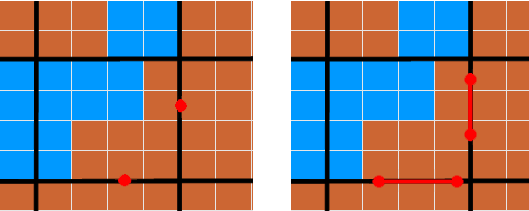
\includegraphics[height=50mm]{91_bilder/clusterArten.png}
\caption[Clustereinteilung auf der Landkarte.]{Vergleich der Clusterarten: Links der Typ Corner, Rechts der Typ Centered}
\label{fig.clusteredMap}
\end{figure}

Nachfolgend wir erl�utert wie das Clustering vonstatten geht, verwendet wird die Custeringart Corner.\\
Nach dem Einteilen der Cluster werden f�r jeden Cluster und einen Nachbar-Cluster aus der Vierer-Nachbarschaft die Verbindungskanten berechnet. Dies kann nat�rlich nur f�r Clusters gemacht werden die auf einem sichtbaren Teil der Landkarte liegen, was zu Begin des Spiel nicht gegeben ist. Deshalb wird der ClusteringTask in jedem Spielzug aufgerufen, in der Hoffnung ein Cluster komplett verbinden zu k�nnen. Sobald eine beliebige Seite eines Clusters berechnet ist, wird diese Aussenkante im Cluster und dem anliegenden Nachbar gespeichert und nicht mehr neu berechnet.

\begin{figure}[H]
\centering
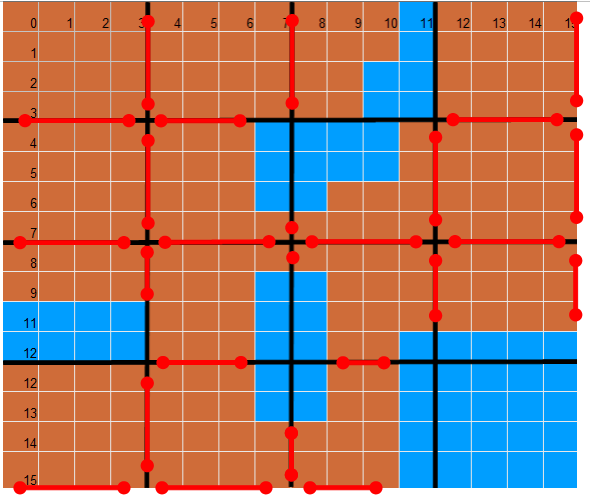
\includegraphics[height=50mm]{91_bilder/clusteredMap2.png}
\caption[Cluster mit berechneten Kanten]{Die Kanten jedes Clusters wurden berechnet}
\label{fig.clusteredMap2}
\end{figure}

Sobald ein Cluster zwei oder mehrere Aussenkanten kennt berechnet er die Innenkanten mit A* welche die Knoten der Aussenkanten verbinden. Dies ergibt nun ein Pfadnetz �ber die Gesamtkarte. Im nachfolgenden Bild sind die Innenkanten (gelb) ersichtlich, die bei den ersten 8 Cluster berechnet wurden.

\begin{figure}[H]
\centering
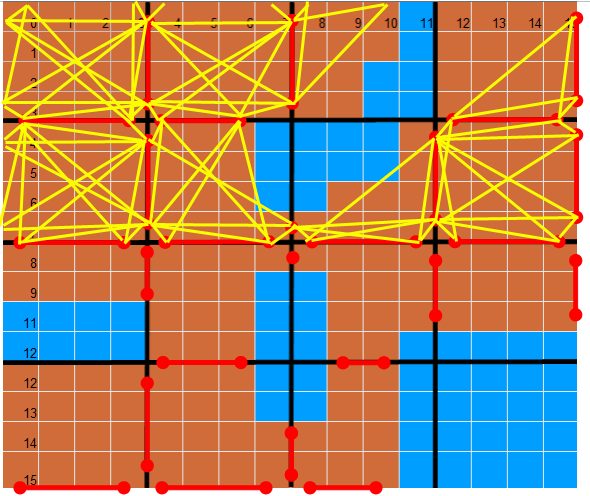
\includegraphics[height=50mm]{91_bilder/clusteredMap3.png}
\caption[Cluster mit Innenkanten]{Darstellung der Innenkanten}
\label{fig.clusteredMap3}
\end{figure}

In der Abbildung \ref{fig.clusteredMap4} wird ein Pfad vom Pixel (3,9) nach (13,9) mittels HPA* gesucht (gr�ne Punkte). Zuerst wird eruiert in welchem Cluster sich das Start- bzw Zielpixel befindet. Danach wird in dem gefundenen Cluster ein Weg zu einem beliebigen Knoten auf der Clusterseite gesucht. Sind diese Knoten erreicht (blaue Pfade), wird nun das vorberechnete Pfadnetz mittels bereits beschrieben A* Algorithmus verwendet um die beiden Knoten auf dem k�rzesten m�glichen Pfad (gelb) zu verbinden. Der resultierende Pfad k�nnte kann nun via Pathsmoothing verk�rzt werden.

\begin{figure}[H]
\centering
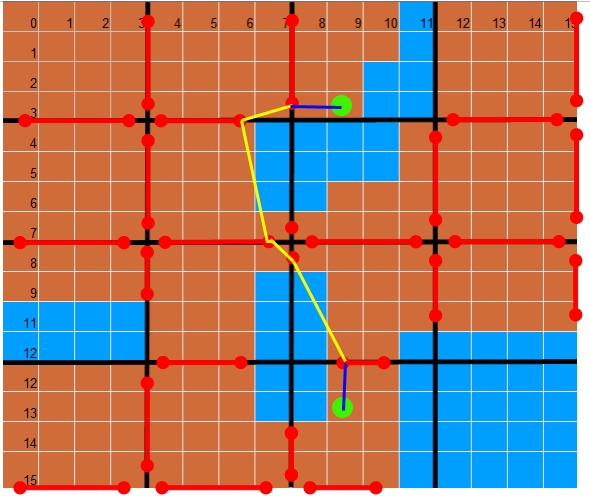
\includegraphics[height=50mm]{91_bilder/clusteredMap4.png}
\caption{Errechneter Weg mittels HPA*}
\label{fig.clusteredMap4}
\end{figure}

Um eine Pfadsuche mit HPA* durchzuf�hren muss ein ClusteringPathFinder instanziert werden. Als Parameter erwartet der Konstruktor die Karte auf welcher das Clustering und die Pfadsuche gemacht wird, sowie die Clustergr�sse (hier: 10) und den Clustertyp. Das Clustering wird mit pf.update() durchgef�hrt. Danach kann die Pfadsuche durchgef�hrt werden. Falls das Clustering auf dem ben�tigten Kartenausschnitt nicht komplett durchgef�hrt werden konnte, weil nicht alle Tiles in einem Cluster sichtbar waren, wird versucht mit A* einen Pfad zu suchen.

\lstset{language=Java, tabsize=4}
\begin{lstlisting}
ClusteringPathFinder pf = new ClusteringPathFinder(map, 10, type);
pf.update();
List<Tile> path = pf.search(PathFinder.Strategy.HpaStar, start, end, -1);
\end{lstlisting}

\subsection{Pfadsuche mittels Influence Map}
\label{subsec:module.Suchalgorithmen.Pfadsuche.WithInfluenceMap}

Die Influence Map, welche wir w�hrend der Bachelorarbeit neu implementiert haben, kann auch f�r die Pfadsuche verwendet werden. Dabei sind die Pfadkosten f�r Gebiete in die vom Gegner kontrolliert sind h�her als f�r neutrale Gebiete und tiefer f�r solche Gebiete die von unseren Ameisen kontrolliert werden. (Details zur Implementierung der InfluenceMap sieh Kapitel TODO) Die Methode getActualCost(...) in der Klasse SearchStrategy wurde erweitert. Falls die Suche mit einer InfluenceMap initialisiert wurde, sind die Kosten nicht eine Einheit pro Pfadtile, sondern k�nnen zwischen 1 (sicheres Gebiet) - 4 (gef�hrliches Gebiet) Einheiten variieren. (Die Pfadkosten d�rfen nicht negativ sein, sonst w�rde der A* Algorithmus nicht mehr korrekt funktionieren.) Die Kosten f�r jeden Pfadabschnitt werden durch die Methode getPathCosts(...) der InfluenceMap berechnet.

\lstset{language=Java, tabsize=4}
\begin{lstlisting}
protected final int getActualCost(Node current, PathPiece piece) {
    int costOfPiece = 0;
    if (useInflunceMap)
        costOfPiece = pathFinder.getInfluenceMap().getPathCosts(piece);
    else
        costOfPiece = piece.getCost();
    return current.getActualCost() + costOfPiece;
}
\end{lstlisting}

Dadurch resultiert ein Pfad der durch sicheres Gebiet f�hrt. Folgende Ausgabe, welche durch einen UnitTest generiert wurde, bezeugt die korrekte Funktionalit�t. Der rote Punkt soll mit dem schwarzen Punkt durch einen Pfad verbunden werden. Auf der Karte sind zudem die eigenen, orangen Einheiten sowie die gegnerischen Einheiten (blau) abgebildet. Jede Einheit tr�gt zur Berechnung der InfluenceMap bei. Pro Tile wird die Sicherheit ausgegeben, negativ f�r Gebiete die vom Gegner kontrolliert werden und positiv in unserem Hoheitsgebiet.

\begin{figure}[H]
\centering
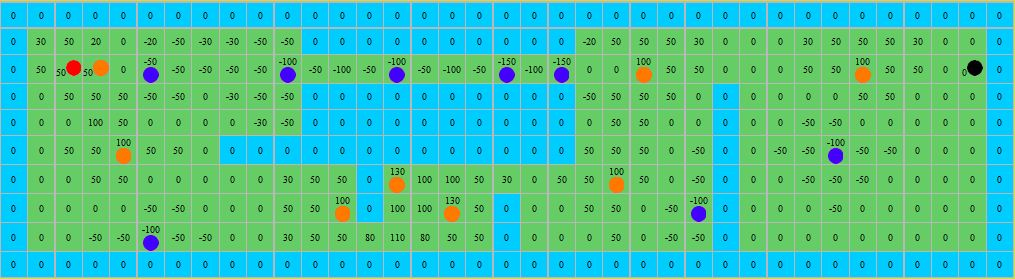
\includegraphics[width=0.99\textwidth]{91_bilder/influenceAStar01.jpg}
\caption{Ausgangslage Pfadsuche mit A* und InfluenceMap}
\label{fig.InfluenceAndPathfinding01}
\end{figure}

Ohne Ber�cksichtigung der InfluenceMap w�rde der A* Algorithmus einen Pfad finden der auf direktem Weg waagrecht zum Zielpunkt f�hrt. Sobald aber die InfluenceMap ber�cksichtigt wird, f�hrt der Pfad nicht mehr auf dem direktesten Weg zum Ziel, sondern nimmt einen Umweg �ber sicheres Gebiet. Unten abgebildet ist der k�rzeste Pfad mit Ber�cksichtigung der InfluenceMap (blau) und ohne InfluenceMap-Ber�cksichtigung (orange). 

\begin{figure}[H]
\centering
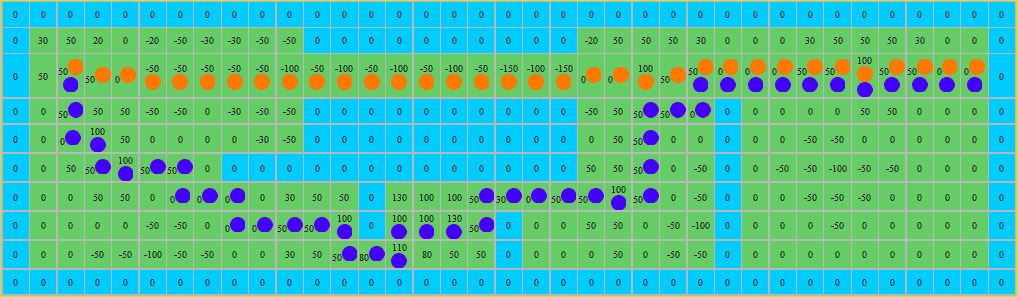
\includegraphics[width=0.99\textwidth]{91_bilder/influenceAStar02.jpg}
\caption{Resultierende Pfade mit und ohne Ber�cksichtigung der InfluenceMap}
\label{fig.InfluenceAndPathfinding02}
\end{figure}

Die Pfadkosten f�r beide Pfade verglichen, legt offen, dass je nach Ber�cksichtigung der InfluenceMap nicht der gleiche Pfad als der 'K�rzeste' von A* gefunden wird.

\renewcommand{\arraystretch}{1.5}
\begin{table}[H]
	\centering
\begin{tabular}{l | r r}
 & Kosten ohne InfluenceMap &Kosten mit InfluenceMap \\
\hline
 Oranger Pfad & \textbf{34} & 110 \\
 Blauer Pfad & 46 & \textbf{106} \\
 \end{tabular}
 \caption{Pfadkosten mit und ohne Ber�cksichtigung der InfluenceMap}
\end{table}
 
\subsection{Pathsmoothing}
\label{subsec:module.Suchalgorithmen.Pfadsuche.Pathsmoothing}

Um unseres Search-Framework zu komplettieren bietet die Pfadsuche auch ein PathSmoothing, das 'Gl�tten' eines Pfades an. Wie im Clustering schon erw�hnt, kann es sein, dass ein Pfad, der von dem HPA* Algorithmus gefunden wurde, nicht zwingend der K�rzeste ist. Die folgende Abbildung veranschaulicht wie der gefundene Pfad von Cluster zu Cluster (weisse Markierung), stets �ber die vorberechneten Verbindungspunkte (blau) verl�uft. Dies ist nicht der optimale Pfad, er kann mit PathSmoothing verk�rzt werden.

\begin{figure}[H]
\centering
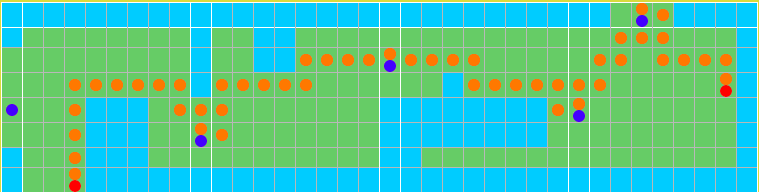
\includegraphics[width=0.99\textwidth]{91_bilder/pathsmoothingOne}
\caption{Der gefundene Pfad mit HPA* Clusteringart Centered, ist nicht der k�rzeste.}
\label{fig.pathsmoothingOne}
\end{figure}

Der Algorithmus des Pathsmoothing ist (vereinfacht) wie folgt definiert. Vom Pfad der gek�rzt werden soll wird ein erster Abschnitt mit der L�nge \textit{size} genommen. Mittels manhattanDistance wird gepr�ft ob eine k�rzere Weg f�r diesen Abschnitt m�glich w�re. Falls ja wird mittels A* ein neuer Pfad gesucht, sonst wird der alte Pfad (\textit{subPath} �bernommen. Dieses Verfahren wird f�r alle nachfolgenden Pfadabschnitte gemacht, bis der ganze Pfad durchlaufen ist.\\
\\
\textbf{Rekursion:} Der beschriebene Algorithmus, hat nicht in jedem Fall den k�rzesten Pfad als Output. So sind zwar alle Pfadabschnitte optimal gek�rzt, es kann aber sein, dass wenn zwei Abschnitte zusammen gef�gt werden, der Pfad nicht mehr der k�rzeste ist. Als Beispiel: Die Wegabschnitt Z�rich-Thun und Thun-Genf m�gen optimal gek�rzt sein. Zusammengef�gt zur Strecke Z�rich-Genf, braucht es den Umweg �ber Thun nicht. Um Umweg zu entfernen wird der Algorithmus rekursiv aufgerufen, indem smoothPath(...) mit einer gr�sseren \textit{size} als Parameter f�r die zusammengesetzten Abschnitte nochmals aufgerufen wird.

\lstset{language=Java, tabsize=4}
\begin{lstlisting}
public List<Tile> smoothPath(List<Tile> path, int size, boolean recursive) {
	int start = 0;
	int current = size;
	List<Tile> smoothedPath = new ArrayList<Tile>();
	// do while the last tile of the smoothed path is the same as in path
	do {
	    List<Tile> subPath = path.subList(start, current);
	    int manDist = map.manhattanDistance(subPath.get(0), subPath.get(subPath.size() - 1)) + 1;	
	    List<Tile> newSubPath = null;
	    if (manDist < subPath.size()) {
	        newSubPath = search(Strategy.AStar, subPath.get(0), subPath.get(subPath.size() - 1), subPath.size() - 1);
	    }
	    if (newSubPath != null) {
	        smoothedPath.addAll(newSubPath);
	        if (recursive && newSubPath.size() < subPath.size()) {
	            smoothedPath = smoothPath(smoothedPath, smoothedPath.size(), true);
	        }
	    } else {
	        smoothedPath.addAll(subPath);
	    }
	    start = current;
	    current = Math.min(current + size, path.size());
} while (!path.get(path.size() - 1).equals(smoothedPath.get(smoothedPath.size() - 1)));

return smoothedPath;
}
\end{lstlisting}

In der n�chsten Abbildung wurde der beschriebene PathSmoothing Algorithmus angewendet, der Pfad konnte einer urspr�nglichen Pfadl�nge   von 50 Tiles (siehe \ref{fig.pathsmoothingOne}) auf eine Pfadl�nge von 40 Tiles reduziert werden.

\begin{figure}[H]
\centering
\includegraphics[width=0.99\textwidth]{91_bilder/pathsmoothingTwo}
\caption{Der gegl�ttete Pfad, nach Anwendung des PathSmoothing-Algorithmus}
\label{fig.pathsmoothingTwo}
\end{figure}%S DONE wieso hpa*
\section{Breitensuche}
\label{subsec:module.Suchalgorithmen.Breitensuche}

Die Breitensuche (engl. breadth-first search (BFS)) war eine der Neuimplementierungen w�hrend der Bachelorarbeit. Wir verwenden diese Suche um die Umgebung einer Ameise oder eines H�gels nach Futter, Gegnern usw. zu scannen. Man k�nnte die BFS auch f�r die Pfadsuche verwenden, dies w�re aber sehr ineffizient. Im Klassendiagramm ist zu sehen auf welchen drei Methoden die Breitensuche aufbaut.

\begin{figure}[H]
\centering
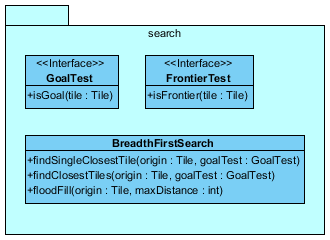
\includegraphics[width=0.7\textwidth]{91_bilder/BFS}
\caption{Breitensuche Klassendiagramm}
\label{fig:BFS}
\end{figure}

TODO FRONTIER TEST fehlt auf dem Bild


Die Breitensuche wurde generisch implementierte, so dass sie vielseitig einsetzbar ist. So k�nnen zum Beispiel mittels 'GoalTest' je nach Anwendungsfall die Tiles beschrieben werden die gesucht sind. Folgende Breitensuche findet die Ameise welche am n�chsten bei einem Food-Tile <r:20,c:16> ist. Die Suche wird initialisiert indem im Konstruktor die Spielkarte mitgegeben wird, welche durchforscht wird. Zus�tzlich gilt die Einschr�nkung das die Breitensuche nur 40 Tiles durchsuchen darf, was einem Radius von zirka 7 Zellen entspricht. Falls keine Ameise gefunden wird gibt der Algorithmus NULL zur�ck.

\lstset{language=Java, tabsize=4}
\begin{lstlisting}
AntsBreadthFirstSearch bfs = new AntsBreadthFirstSearch(Ants.getWorld());
Tile food = new Tile(20,16);
Tile antClosestToFood = bfs.findSingleClosestTile(food, 40, new GoalTest() {
      @Override
      public boolean isGoal(Tile tile) {
          return isAntOnTile(tile);
      }
  });
\end{lstlisting}

Es ist auch m�glich mehrere Tiles zur�ck zu bekommen. Dazu wird die Methode \textit{findClosestTiles(...)} aufgerufen.\\
\\
Der gleiche Algorithmus kann aber auch alle passierbaren Tiles in einem gewissen Umkreis zur�ckgeben. Dies haben wir unter anderem beim Initialisieren der DefendHillMission verwendet. Wir berechnen beim Erstellen der Mission die passierbaren Zellen rundum den H�gel. Runde f�r Runde pr�fen wir diese Tiles auf gegnerische Ameisen um die entsprechenden Verteidigungsmassnahmen zu ergreifen. Der Parameter controlAreaRadius2 definiert den Radius des 'Radars' und kann je nach Profile unterschiedlich eingestellt werden.

\lstset{language=Java, tabsize=4}
\begin{lstlisting}
public DefendHillMission(Tile myhill) {
    this.hill = myhill;
    BreadthFirstSearch bfs = new BreadthFirstSearch(Ants.getWorld());
    tilesAroundHill = bfs.floodFill(myhill, controlAreaRadius2);
}
\end{lstlisting}


Um die Aufrufe der Suche im Ants-Umfeld einfacher zu gestalten haben wir die Breitensuche f�r unseren Bot mit folgenden selbst-sprechenden Methoden erweitert.

\begin{figure}[H]
\centering
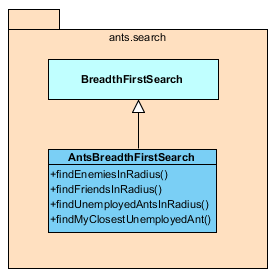
\includegraphics[width=0.5\textwidth]{91_bilder/BFSants}
\caption{Breitensuche Ants-spezifisch}
\label{fig:BFSants}
\end{figure}



\subsection{Barrier (Sperre)}
\label{subsec:module.Suchalgorithmen.Breitensuche.Barrier}

Eine Erweiterung der Breitensuche erm�glicht uns eine Sperre in der Umgebung eines Ortes zu finden. Diese Verwenden wir in der DefendHillMission zum Verteidigen des eigenen H�gels. Es kann nur eine Sperre (engl. Barrier) gefunden werden wenn das Gel�nde dazu passt. Die Abbildung zeigt einen gefundene Sperre. Auf dieser H�he wird der H�gel verteidigt.

\begin{figure}[H]
\centering
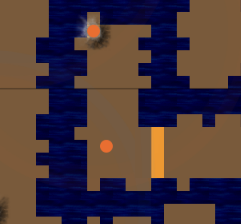
\includegraphics[width=0.5\textwidth]{91_bilder/barrier}
\caption{Auf der orangen Sperre werden die Ameisen zur Verteidigung des H�gel positioniert.}
\label{fig:search.barrier}
\end{figure}

Der Algorithmus verbirgt sich in der Methode \textit{getBarrier(...)}. Diese wird mit den Parametern \textit{tileToProtect}: Ort der durch eine Sperre gesch�tzt werden soll, \textit{viewRadiusSquared}: den Sichtradius der Einheiten, den die Sperre soll weiter entfernt sein als der Sichtradius, damit die gegnerischen Einheiten nicht sehen was sich dahinter verbirgt. Der dritte Parameter \textit{maximumBarrierSize} definiert welche Breite die Sperre maximal haben darf.

\lstset{language=Java, tabsize=4}
\begin{lstlisting}
public Barrier getBarrier(final Tile tileToProtect, int viewRadiusSquared, int maximumBarrierSize) {
	int amount = BFS for getting the amount of tiles in view radius around the location to defend.
	Barrier smallestBarrier = null;
	List<Tile> tiles = get (amount + 30) tiles around the location to defend.
	
	// for loop start at the first tile not in view radius
	for(int i = amount;i<tiles.size(); i++){       
		Tile t = tiles.get(i);
		
		//vertical check
		if(!barrierVerticalInvalid.contains(t)){
			Barrier b = get vertical barrier on position of Tile t
			if(b is smaller than 5 Tiles && smaller than smallestBarrier){
				if(is barrier the only exit out of the location to defend){
						smallestBarrier = b;
				}else{
						 //add all tiles of the invaild barrier
						barrierVerticalInvalid.add(b.getTiles());
				}    					      		
			}else{
				 //add all tiles of the invaild barrier
				barrierVerticalInvalid.add(b.getTiles());
			}
		}
		
		//horizontal check
		if(!barrierHorizontalInvalid.contains(t)){
			Barrier b = get horiontal barrier on position of Tile t
			if(b is smaller than 5 Tiles && smaller than smallestBarrier){
				if(is barrier the only exit out of the location to defend){
						smallestBarrier = b;
				}else{
						 //add all tiles of the invaild barrier
						barrierHorizontalInvalid.add(b.getTiles());
				}    					      		
			}else{
				//add all tiles of the invaild barrier
				barrierHorizontalInvalid.add(b.getTiles());
			}
		}	
	}
}
\end{lstlisting}

Dank dem Abspeichern der ung�ltigen Tiles aller zu breiten Sperren in die Listen \textit{barrierHorizontalInvalid} und \textit{barrierVerticalInvalid} konnte der Algorithmus markant schneller gemacht werden. F�r diese Tiles muss nicht nochmals eine Sperre berechnet werden. Auch die if-Abfrage \textit{barrier is the only exit out of the location to defend} muss nicht mehr oft aufgerufen werden, den hinter dieser Abfrage steht n�mlich wiederum ein Test mit der Breitensuche. Dieser zus�tzliche Test mit der Breitensuche ist viel teurer als das Zwischenspeichern der Tiles aus welchen keine g�ltige Sperre gemacht werden konnte.\\
\\
Im Nachhinein hat sich ergeben, dass nicht unbedingt die schmalste Sperre die Beste w�re, sondern jede bei welche der Gegner, gel�ndebedingt, weniger Einheiten aufstellen kann. So w�re in Abbildung \ref{fig:search.barrier} eine Sperre zwei Zellen �stlicher besser, den der Gegner k�nnte beim Angriff nur mit vier Einheiten vorr�cken, die Verteidigung w�re aber mit sechs Einheiten auf einer Linie deutlich st�rker. Die Zeit hat aber hier leider nicht gereicht, den Algorithmus weiter zu verfeinern.%S DONE OK
\chapter{Strategie}
\label{sec:module.Strategie}%S DONE OK 
\chapter{Ants}
\label{sec:module.Ants}

Alle Klassen im Ants Package sind spezifisch f�r die Ants AI Challenge und machen das Ger�st unseres \gls{Bot}s aus. Nachfolgend wird deren Aufbau erl�utert.

\section{State-Klassen}
\label{sec:module.Ants.State}

\begin{figure}[H]
\centering
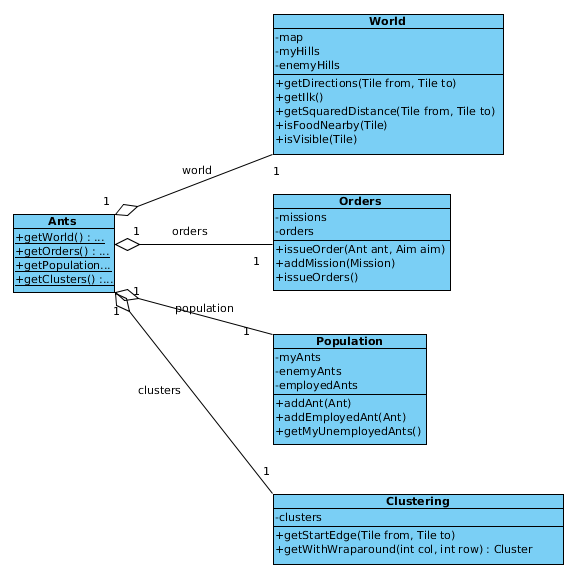
\includegraphics[width=0.7\textwidth]{91_bilder/State}
\caption{State-Klassen (vereinfacht)}
\label{fig:StateClasses}
\end{figure}

Abbildung \ref{fig:StateClasses} zeigt eine \"{U}bersicht �ber der Spielzustands-Klassen. F�r das Diagramm wurden lediglich die wichtigsten Methoden und Attribute ber�cksichtigt. Die State-Klassen implementieren alle das Singleton-Pattern.

\subsection{Ants}
\label{sec:module.Ants.State.Ants}
Die Ants Klasse ist die zentrale State-Klasse. Sie bietet auch einfachen Zugriff auf die anderen State-Klassen. Urspr�nglich hatten wir alle Methoden, die mit dem Zugriff auf den Spielzustand zu tun hatten, direkt in der Ants Klasse implementiert, haben aber schnell gemerkt, dass das unhandlich wird. Die Ants Klasse dient jetzt vor allem als Container f�r die anderen State-Klassen und implementiert nur noch einige Methoden, die Zustands�nderungen in verschiedenen Bereichen vornehmen.

\subsection{World}
\label{sec:module.Ants.State.World}
Die World Klasse enth�lt Informationen zur Spielwelt und erweitert die AbstractWrapAroundMap aus der AI-Tools API. Hier wird die Karte abgespeichert, in der f�r jede Zelle die aktuell bekannten Informationen festgehalten werden. Das beinhaltet die Sichtbarkeit der Zelle und was die Zelle aktuell enth�lt (Ameise, Nahrung, Wasser, ...). Ausserdem werden Listen gef�hrt, wo sich die eigenen und die bekannten gegnerischen H�gel befinden. Die Klasse bietet Methoden zur Distanzberechnung und gibt Auskunft �ber einzelne Zellen, beispielsweise ob sich Nahrung in der Umgebung einer bestimmten Zelle befindet. Zudem sind die wichtigsten Methoden des SearchableMap Interfaces (\texttt{getSuccessors...()}) hier implementiert.

\subsection{Orders}
\label{sec:module.Ants.State.Orders}
In der Orders Klasse wird �ber Befehle und Missionen der einzelnen Ameisen Buch gef�hrt. In der Liste der Befehle wird zwischengespeichert, welche Ameise welche Bewegung im aktuellen Spielzug macht. Zu Beginn des Spielzuges wird diese geleert, dann von den Tasks und Missionen mit Befehlen belegt, und am Schluss des Spielzuges werden die Befehle der Spielschnittstelle �bergeben. Die Liste der Missionen ist zug�bergreifend gef�hrt, da eine Mission �ber mehrere Spielz�ge verlaufen kann. Das zentrale Verwalten der Befehle und Missionen dient dazu, sicherzustellen, dass keine widerspr�chlichen Befehle ausgegeben werden wie: Mehrere Befehle f�r eine Ameise, gleiche Ziel-Koordinaten f�r mehrere Ameisen, eine Ameise ist mehreren Missionen zugeteilt etc..

\subsection{Population}
\label{sec:module.Ants.State.Population}
Die Population Klasse dient der Verwaltung der eigenen und der gegnerischen Ameisen-V�lker. Hier werden die Ameisen mit ihren aktuellen Aufenthaltsorten festgehalten. Wenn f�r eine Ameise ein Befehl ausgegeben wird, wird die Ameise als besch�ftigt markiert. \"{U}ber die Methode \texttt{getMyUnemployedAnts()} kann jederzeit eine Liste der Ameisen abgefragt werden, die f�r den aktuellen Zug noch keine Befehle erhalten haben und f�r neue Aufgaben zur Verf�gung stehen. Die Population Klasse f�hrt zudem Buch �ber die verf�gbaren Ressourcen pro Aufgabentyp und stellt sicher, dass kein Aufgabentyp mehr Ressourcen beansprucht, als ihm zugeteilt sind. (s. Kapitel \ref{sec:module.resourceMgmt})


\section{Spiel-Elemente (Ants-Spezifisch)}
\label{sec:module.Ants.State.Entities.Ants}

\begin{figure}[H]
\centering
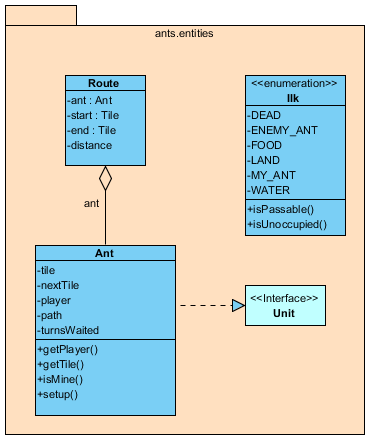
\includegraphics[width=0.5\textwidth]{91_bilder/antsEntities}
\caption{Ants-spezifische Elemente der Spielwelt (vereinfacht)}
\label{fig:antsEntities}
\end{figure}

Abbildung \ref{fig:antsEntities} zeigt die wichtigsten Klassen, die die Elemente des Spiels repr�sentieren. Der \"Ubersichtlichkeit wegen wurden nur die wichtigsten Attribute und Operationen in das Diagramm aufgenommen.

\subsection{Ant}
\label{sec:implementation.Entities.Ant}
Eine Ant (Ameise) geh�rt immer zu einem Spieler; �ber die Methode \texttt{isMine()} k�nnen unsere eigenen Ameisen identifiziert werden. 
Die Ant Klasse implementiert das Interface Unit aus der AITools-API, welches eine Abstraktion bietet, die die Verwendung der Ameisen in den generischen Modulen erlaubt.
Eine Ameise weiss jeweils, in welcher Zelle sie steht. Das Feld \texttt{nextTile} dient der Verfolgung einer Ameise �ber mehrere Z�ge. Der Wert des Feld wird jeweils gesetzt, wenn der Ameise ein n�chster Zug zugewiesen wird. Im n�chsten Spielzug wird die Position der Ameise durch diese Information aktualisiert.

\subsection{Route}
\label{sec:implementation.Entities.Route}
Eine Route repr�sentiert eine einfache Verbindung zwischen zwei \gls{Tile}s. Die Distanz wird zwischen den \gls{Tile}s wird mit der Luftliniendistanz gemessen.

\subsection{Ilk}
\label{sec:implementation.Entities.Ilk}
Ilk ist der Typ einer Zelle. Der Ilk einer \gls{Tile}-Instanz gibt an, was sich gerade in der Zelle befindet. Dies kann ein Gel�ndetyp sein, wenn die Zelle nicht besetzt ist, oder es kann eine Ameise, Nahrung, oder ein H�gel sein; in diesem Fall ist der Gel�ndetyp implizit ''Land``, da Wasser-\gls{Tile}s nicht besetzt sein k�nnen. Die Ilk-Enumeration bietet Hilfsmethoden, um festzustellen, ob eine Zelle passierbar oder besetzt ist.
%S DONE OK
\section{Aufbau Bot}
\label{sec:module.AufbauBot}

Dieses Kapitel beschreibt die Klassenhierarchie unserer Bot Implementation.

\subsection{Klasse Bot}
\label{sec:module.Bot.Bot}

\begin{figure}[H]
\centering
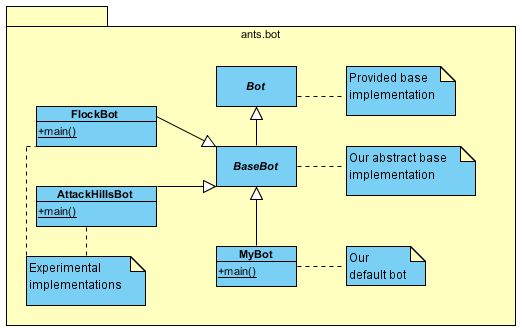
\includegraphics[width=0.7\textwidth]{91_bilder/antsBot}
\caption[Bot Klassenhierarchie]{Vererbung der Bots}
\label{fig:antsBot}
\end{figure}

Als Basis f�r unsere Bot Implementation haben wir den Beispiel-Bot (Klasse Bot.java) verwendet, der im Java-Starter-Package enthalten ist. Das Starter-Package kann von der AI-Challenge Website\footnote{http://aichallenge.org/ants\_tutorial.php} heruntergeladen werden. Der Bot erweitert die Klassen AbstractSystemInputReader und AbstractSystemInputParser, welche die Interaktion mit der Spielengine �ber die System-Input/Output Streams kapseln. F�r eine optimierte L�sung k�nnte der Bot auch angepasst werden, indem er selber auf die Streams zugreift. Im Rahmen dieser Arbeit erschien uns das nicht n�tig. Die Klasse Bot dient als Grundlage f�r die Klasse BaseBot, welcher wiederum Grundlage ist f�r die Klasse MyBot, wie Abb. \ref{fig:antsBot} illustriert.
Die Klasse BaseBot wurde in erster Linie eingef�hrt, um m�glichst einfach verschiedene Bot Implementierungen zu Testzwecken schreiben zu k�nnen (s. Kapitel \ref{sec:testCenter.Testbots}).

Die Bot Implementierungen verf�gen jeweils �ber die Einsprungs-Methode \texttt{main()}, die im einfachsten Fall aus einer einzelnen Zeile besteht (z.B. \texttt{new FlockBot().readSystemInput();}). Listing \ref{lst:mainMethod} zeigt die \texttt{main()}-Methode von MyBot.

\lstset{language=Java, tabsize=4}
\begin{lstlisting}[caption=Main-Methode von MyBot, label=lst:mainMethod]
public static void main(String[] args) throws IOException {
        // we only support one arg, and that is assumed to be the profile name
        String profile = args.length == 1 ? args[0] : null;
        initLogging(profile);
        new MyBot(profile).readSystemInput();
    }
		
\end{lstlisting}

\subsection{Klasse BaseBot}
\label{sec:module.Bot.BaseBot}

Die abstrakte Klasse BaseBot erbt von Bot. Hier haben wir die Struktur unseres Spielzuges definiert.

\subsubsection{Ablauf eines Zugs} 
\label{sec:implementation.Bot.Turn}

\begin{figure}[H]
\centering
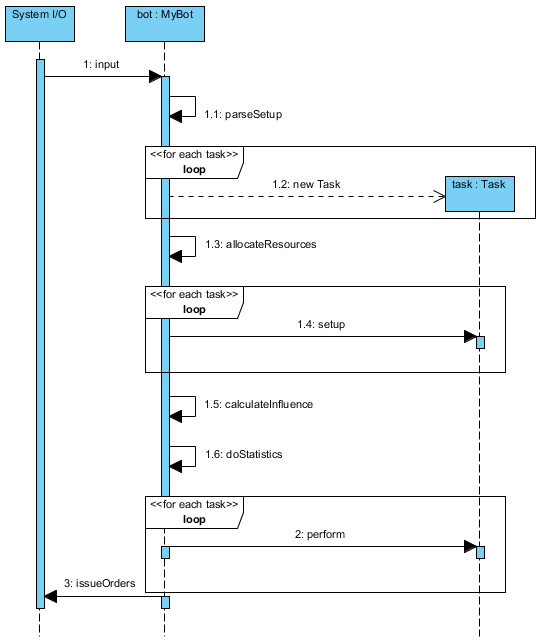
\includegraphics[width=0.8\textwidth]{91_bilder/FirstTurn}
\caption{Ablauf des ersten Zugs des Spiels}
\label{fig:firstTurn}
\end{figure}

Abbildung \ref{fig:firstTurn} zeigt den Ablauf des ersten Zugs, w�hrend Abbildung \ref{fig:turn} den Ablauf aller weiteren Z�ge zeigt. 

\begin{figure}[H]
\centering
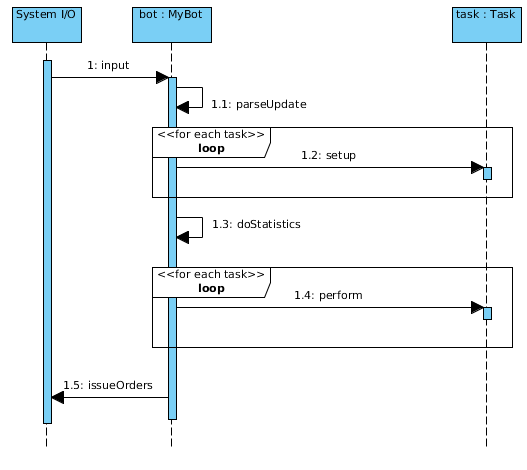
\includegraphics[width=0.8\textwidth]{91_bilder/Turn}
\caption{Ablauf der weiteren Z�ge des Spiels}
\label{fig:turn}
\end{figure}

Jeder Zug beginnt mit dem Einlesen des Inputs vom SystemInputStream. Wenn der Bot das Signal ''READY`` (1. Zug) oder ''GO`` (alle weiteren Z�ge) erh�lt, kann er den gesammelten Input verarbeiten (Methode \texttt{parseSetup()} respektiv \texttt{parseUpdate()}). Danach wird die eigentliche Logik des Bots in der Methode \texttt{doTurn(...)} ausgef�hrt.

Im 1. Zug werden dabei Instanzen der Tasks erstellt. Abgesehen davon unterscheidet sich der 1. Zug von diesem Punkt an nicht mehr von allen nachfolgenden Z�gen. Die Tasks werden vorbereitet (Aufruf der jeweiligen \texttt{setup()} Methode). Danach werden einige statistische Werte aktualisiert und in jedem 10. Zug auch geloggt. Dann werden die Tasks in der definierten Reihenfolge aufgerufen. Hier wird der L�wenanteil der Zeit verbracht, denn die Tasks enthalten die eigentliche Logik unserer Ameisen.

Zum Schluss werden dann mit \texttt{issueOrders()} die Z�ge der Ameisen �ber den SystemOutputStream an die Spielengine �bergeben. Im Code sieht das ganze folgendermassen aus.

\lstset{language=Java, tabsize=4}
\begin{lstlisting}[caption=Der Ablauf des Spielzugs, label=lst:ablaufspielzug]
@Override
/*
 * This is the main loop of the bot. All the actual work is
 * done in the tasks that are executed in the order they are defined.
 */
public void doTurn() {
		// write current turn number, ants amount into the log file.
	addTurnSummaryToLogfiles();
		// new calculation of the influence map
	calculateInfluence();
		// write some statistics about our population
	doStatistics();
		// initialize the task (abstract method); this is implemented in the subclasses
	initTasks();
		// execute all task (main work to do here)
	executeTask();
		// write all orders to the output stream
	Ants.getOrders().issueOrders();
		// log all ants which didn't get a job.
	logUnemployedAnts();
}
\end{lstlisting}


\subsection{Klasse MyBot}
\label{sec:module.Bot.MyBot}

Wie bereits im Listing \ref{lst:ablaufspielzug} ersichtlich, ist die Methode \texttt{initTasks()} in BaseBot abstrakt und muss von MyBot implementiert werden. \texttt{initTasks()} definiert welche Tasks, oder besser gesagt F�higkeiten der Bot hat. Dies wurde ausgelagert, da nicht nur MyBot von BaseBot erbt, sondern auch weitere Bots, die wir zu Testzwecken erstellt haben um bestimmte Funktionalit�ten isoliert zu testen. (Siehe dazu \ref{sec:testCenter.Testbots}) Weiter wird in der \texttt{main()}-Methode von MyBot \texttt{initLogging(...)} aufgerufen. Hier definieren wir, welche Logkategorien mit welchem Loglevel ins Logfile geschrieben werden. (Mehr zum Thema Logging siehe Kapitel \ref{sec:module.Logging}). Je nach Modul, das gerade getestet wird kann so die Anzahl Logeintr�ge justiert werden.\\
MyBot initialisiert die folgenden aufgef�hrten Tasks; es sind die Tasks, die sich im Lauf der Arbeit bew�hrt haben. Die detaillierte Beschreibung der Tasks ist im nachfolgenden Kapitel \ref{sec:module.Tasks} zu finden.

\begin{itemize}
		\item GatherFoodTask
		\item AttackHillsTask
		\item DefendHillTask
		\item ExploreTask
		\item ClearHillTask
		\item CombatTask
		\item ClusteringTask
\end{itemize}%S DONE OK
\section{Tasks}
\label{sec:module.Tasks}

\begin{figure}[bth]
\centering
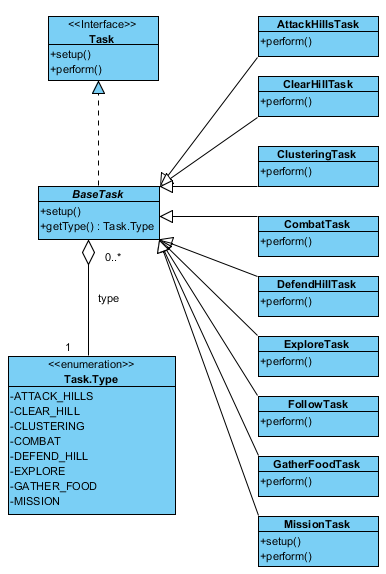
\includegraphics[width=0.5\textwidth]{91_bilder/Tasks}
\caption{Tasks}
\label{fig:tasks}
\end{figure}
Zu Beginn des Projekts haben wir die wichtigsten Aufgaben einer Ameise identifiziert. Diese Aufgaben wurden als Tasks in eigenen Klassen implementiert. Das Interface Task\footnote{Das Interface ist im Code unter ants.tasks.Bot.Java auffindbar.} definiert eine setup()-Methode welche den Task initiiert, sowie eine perform()-Methode welche den Task ausf�hrt. Im Programm werden die Tasks nach deren Wichtigkeit ausgef�hrt, was auch der nachfolgenden Reihenfolge entspricht. Jedem Task stehen nur die unbesch�ftigten Ameisen zur Verf�gung, d.h. jene welchen noch keine Aufgabe zugeteilt wurde.

\subsubsection{MissionTask}
\label{subsec:implementation.Tasks.MissionTask}
Dieser Task pr�ft alle aktuellen Missionen auf deren G�ltigkeit, beispielsweise ob die Ameise der Mission den letzten Zug �berlebt hat und die Mission weiterf�hren kann. Falls g�ltig, wird der n�chste Schritt der Mission ausgef�hrt.

\subsubsection{GatherFoodTask}
\label{subsec:implementation.Tasks.GatherFoodTask}
F�r jedes Food-Tile werden in einem definierbaren Radius r die n�chsten Ameisen bestimmt. Danach wird nach aufsteigender Luftliniendistanz mit dem Pfadsuchalgorithmus SIMPLE (s. Abschnitt \ref{subsec:implementation.Pfadsuche.Simple}) oder -- falls dieser keinen Pfad gefunden hat -- mit A* eine passierbare Route gesucht. Wenn ein Pfad existiert, kann mit der Ameise und dem Food-Tile eine GatherFoodMission erstellt werden, welche die Ameise zum Food-Tile f�hrt. Zu jedem Food-Tile wird immer nur eine Ameise geschickt.

\subsubsection{AttackHillsTask}
\label{subsec:implementation.Tasks.AttackHillsTask}
Sobald gegnerische Ameisenhaufen sichtbar sind, sollen diese angegriffen werden. Das Zerst�ren eines gegnerischen Haufens ist wie erw�hnt 2 Punkte wert. Die Kriterien, nach denen eine Pfad zum gegnerischen Haufen gesucht wird, sind die selben wie beim GatherFoodTask, ausser dass mehrere Ameisen das Ziel angreifen k�nnen. Es wird eine AttackHillMission erstellt.

\subsubsection{CombatTask}
\label{subsec:implementation.Tasks.CombatTask}
Beim Angriffstask wird berechnet ob wir in einem Kampfgebiet (definiert �ber den Sichtradius einer Ameise) die �berhand, d.h. mehr Ameisen platziert haben. Falls ja, wird die gegnerische Ameise angegriffen.

\subsubsection{DefendAreaTask}
\label{subsec:implementation.Tasks.DefendAreaTask}
Dieser Task w�re vogesehen um eine Region wie zum Beispiel den eigenen Ameisenh�gel zu sch�tzen. Dieser Task wurde im Zuge dieser Arbeit nicht implementiert.

\subsubsection{ExploreTask}
\label{subsec:implementation.Tasks.ExploreTask}
F�r alle noch unbesch�ftigten Ameisen wird mittels ManhattanDistance der n�chste Ort gesucht, der noch nicht sichtbar, also unerforscht ist. Falls ein Pfad mittels Pfadsuchalgorithmus gefunden wird, wird eine ExploreMission (s. Abschnitt \ref{sec:implementation.Missionen}) erstellt. Die Ameise wird den gefundenen Pfad in den n�chsten Spielz�gen ablaufen.

\subsubsection{FollowTask}
\label{subsec:implementation.Tasks.FollowTask}
Der FollowTask ist f�r Ameisen angedacht welche aktuell keine Aufgabe haben. Diese Ameisen sollen einer nahe gelegenen, besch�ftigten Ameise folgen, damit diese nicht alleine unterwegs ist.

\subsubsection{ClearHillTask}
\label{subsec:implementation.Tasks.ClearHillTask}
Dieser Task bewegt alle Ameisen, welche neu aus unserem H�gel ''schl�pfen``, vom H�gel weg. So werden nachfolgende Ameisen nicht durch diese blockiert.

\subsubsection{ClusteringTask}
\label{subsec:implementation.Tasks.ClusteringTask}
Der ClusteringTask wird als Vorbereitung f�r den HPA* Algorithmus verwendet. Hier wird f�r alle sichtbaren Kartenregionen ein Clustering vorgenommen. Das Clustering wird im Kapitel \ref{subsec:implementation.Pfadsuche.HPAstar} im Detail beschreiben.
%S DONE OK
\section{Missionen}
\label{sec:module.Missionen}

Missionen sind das Herzst�ck unserer Arbeit. Eine Mission dauert �ber mehrere Spielz�ge und berechnet f�r jede teilnehmende Ameise welches ihr n�chster Move ist. Nachfolgende Darstellung zeigt, dass alle Missionen von der abstrakten BaseMission abstammen und die BaseMission das Interface Mission implementiert. Die Lebensdauer einer Mission h�ngt davon ab, ob sie ihr Ziel erreicht oder ob sie schon f�hrer abgebrochen werden muss. Ziel und Abbruchbedingungen sind je nach Mission unterschiedlich und werden im jeweiligen Abschnitt erkl�rt.

\begin{figure}[H]
\centering
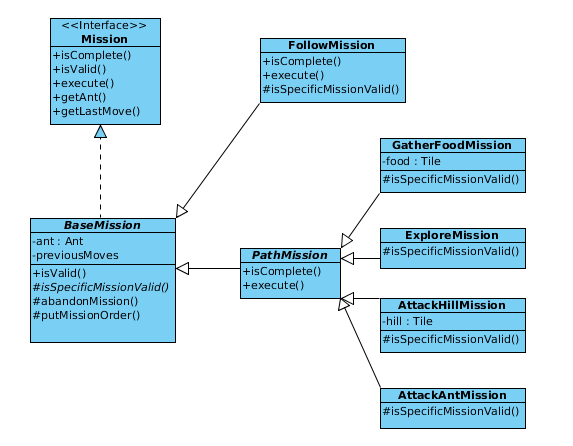
\includegraphics[width=0.9\textwidth]{91_bilder/Missions}
\caption{Missionen und ihre Hierarchie}
\label{fig:missions}
\end{figure}


\subsection{BaseMission}
\label{subsec:module.Mission.BaseMission}

Diese Klasse hat zwei Verwendungszwecke, erstens Implementiert sie die von Interface Mission vorgegebene Methoden und zweitens stellt sie Funktionen zur Verf�gung die von spezifischen Missionen verwendet werden. Die wichtigsten sind hier mit Erkl�rung aufgelistet.

\begin{itemize}
	\item  \textbf{abandonMission():} Abbrechen der Mission
	\item  \textbf{addAnt():} Ameise der Mission hinzuf�gen, in der Population als besch�ftigt markieren.
	\item  \textbf{doAnyMove(Ant a):} F�r die mitgegebene Ameise irgendein Zug in eine der vier Richtung bestimmen.
	\item  \textbf{doMoveInDirection(Ant ant, Tile target):} Ein Zug in eine bestimmte Richtung bestimmen.}
	\item  \textbf{gatherAnts(...):} Ameisen f�r die Mission rekrutieren. Anzahl Ameisen wird als Parameter mitgegeben. }
	\item  \textbf{moveToNextTileOnPath(Ant a):} Bewegt die Ameise ein Pfadst�ck weiter auf dem, der Ameisen zugewiesen, Pfad.}
	\item  \textbf{putMissionOrder(...):} Wurde ein Befehl f�r die Ameise gefunden wird er der Klasse Orders (Verwaltung der Befehle) mitgeteilt.}
	\item  \textbf{releaseAnts(int amount):} Ameisen vo der Mission entlassen. 
	\item  \textbf{checkEnviroment(...):} Mittels Breitensuche wird die Umgebung der Ameise nach eigenen H�gel, gegnerischen H�gel, gegnerischen Ameisen und Futterzellen gescannt. Je nach Mission wird beim Fund eines solchen Objekt die Mission abgebrochen, oder die Ameise von der Mission entlassen.
\end{itemize}
\\
\\
Nachfolgend werden die spezifischen Missionen erl�utert. Tabellearisch werden die Eigenschaften der Missionen aufgelistet, danach folgen detailiierte Infomationen zur Mission.


\subsection{PathMission}
\label{subsec:module.Mission.PathMission}

Precondition: -\\
Creator: (Ersteller): CombatTask, oder ExploreMission\\
Postcondition: Pfad vollst�ndig abgelaufen\\
Max. Ants (Maximale Anzahl Ameisen): 1\\
Max. Missionen: unbegrenzt\\
Valid (G�ltigkeit): siehe ExploreMission bzw. CombatTask\\
Gather Ants (Ameisen rektrutieren): Nicht m�glich\\
Release Ants (Ameisen entlassen): Nicht m�glich\\
\\
Die Pathmission ist eine abstrakte Klasse die von ExploreMission und als anonyme Klasse im CombatTask implementiert wird. Die einzige Funktionalit�t die angeboten wird ist, eine Ameise die der Initialisierung mit Pfad mitgegeben wird, auf diesem definierten Pfad zu bewegen.

\subsection{AttackHillMission}
\label{subsec:module.Mission.AttackHillMission}

Precondition: Gegnerischer H�gel sichtbar\\
Creator: AttackHillsTask\\
Postcondition: Gegnerischer H�gel erobert\\
Max. Ants: unbegrenzt\\
Max. Missionen: Je gegnerischen H�gel eine Mission\\
Valid: solange gegnerischer H�gel nicht zerst�rt ist.\\
Gather Ants: pro Zug max. 5 Ameisen, die im Umkreis von 25 Tiles des gegnerischen H�gel sind.\\
Release Ants: Sicheres Food Tile in der N�he. Eigener H�gel in der N�he der Unterst�ztung braucht. Wenn Mission im Status ControlHill ist werden alle Ameisen entlassen ausser zwei. Diese kontrollieren den H�gel.\\
\\
Diese Mission unterscheidet zwischen drei verschiedenen Modi. Der Modus wird zu Beginn jeder Runde durch die Methode determineState() definiert.\\
\\
\textbf{ControlEnemyHill}\\
Status ist aktiv wenn, 2 oder mehr eigene Ameise in der N�he des gegnerischen H�gel sind. Der Gegner aber nur eine Amesise zur Verteidigung hat.\\
Hier werden alle Ameisen ausser die zwei zum gegnerischen H�gel am n�chsten liegenden Ameisen aus der Mission entlassen. Die �brigen zwei Ameisen positionieren sich auf einer der vier diagonal gelegenen Zellen. Soblad die Ameisen positioniert sind, fressen Sie alle gegnersichen Ameisen die neu aus dem H�gel schl�pfen. Der Gegner kann sich so nur durch Ameisen vermehren die aus einem anderen H�gel schl�pfen. (Die Ameisen schl�pfen zuf�llig aus einem H�gel) Der H�gel wird erst zerst�rt wenn das Spiel endet, oder sich der Gegner mit anderen Ameisen dem H�gel n�hert.

\begin{figure}[H]
\centering
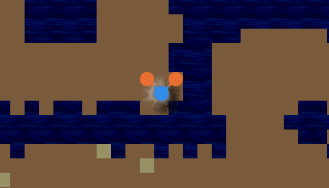
\includegraphics[height=40mm]{91_bilder/ControlEnemyHill}
\caption{Ein gegnerischer H�gel wird durch unsere Ameisen (orange) kontrolliert.}
\label{fig:ControlEnemyHill}
\end{figure}

\textbf{DestroyHill}\\
Status ist aktiv wenn, Spiel 5 Z�ge vor Spielende ist\\
Wenn dieser Modus eintrifft ist das Spiel fast zu Ende. Deshalb wird versucht mit der Brechstange den H�gel zu erobern indem die Ameisen auf dem k�rzesten Weg Richtung gegnerischen H�gel geschickt werden.\\
\\
\textbf{AttackEnemyHill}\\
Status ist aktiv in allen anderen F�llen\\
Alle Angreifer werden nach ihrer Lage in Gruppen zusammen gefasst. F�r diese Gruppe wird ein Pfad zum gegnerischen H�gel berechnet. Falls der Pfad l�nger ist als 5 Tiles wird ein Meilenstein (Milestone) definiert. Nun werden mittels Breitensuche die Gegner zwischen dem Meilenstein und der Gruppe ermittelt. Mit dieser Ausgangslage wird eine AttackingCombatPositioning Klasse initialisert und die Gruppe, die gegnerischen Ameisen sowie der Meilenstein als Ziel mitgegeben. Die Klasse berechnet die Z�ge f�r die Gruppe. (Details siehe \ref{sec:module.CombatSituation}
       
\begin{figure}[H]
\centering
\includegraphics[height=40mm]{91_bilder/AttackHill}
\caption{Die erste zweier Gruppe ist in Kampfstellung. 4 weitere Ameisen r�cken zur Front auf.}
\label{fig:AttackHill}
\end{figure}

\subsection{DefendHillMission}
\label{subsec:module.Mission.DefendHillMission}

Precondition: Keine, Mission wird zu Beginn des Spiels erstellt.\\
Creator: DefendHillTask\\
Postcondition: Gegnerischer H�gel ist erobert.\\
Max. Ants: unbegrenzt\\
Max. Missionen: Je eigener H�gel eine Mission\\
Valid: solange eigener H�gel nicht erobert ist.\\
Gather Ants: Mission soll immer mehr Verteidiger haben als Angreifer sich dem H�gel n�hern.\\
Release Ants: Keine Angreifer in Sicht, werden die Ameisen (nicht alle) entlassen.\\
\\
TODO

\subsection{ExploreMission}
\label{subsec:module.Mission.ExploreMission}

Precondition: - \\
Creator: ExploreTask\\
Postcondition: Definerter Pfad zum Erkunden ist abgelaufen.\\
Max. Ants: 1\\
Max. Missionen: unbegrenzt\\
Valid: Solange Ameise ein g�ltiger Pfad hat.\\
Gather Ants: nicht m�glich\\
Release Ants: nicht m�glich\\
\\
Die Ameise l�uft den vom ExploreTask vorgegebenen Pfad ab. Die Mission wird abgebrochen, wenn Futter in der N�he ist, wenn ein gegnerischer H�gel oder gegnerische Ameisen auftauchen oder wenn ein eigener H�gel in der N�he Hilfe braucht.

\begin{figure}[H]
\centering
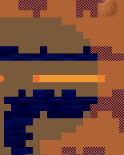
\includegraphics[height=40mm]{91_bilder/exploreMission}
\caption{Eine Ameise auf einer ExploreMission bewegt sich in Richtung Fog Of War}
\label{fig:exploreMission}
\end{figure}

\subsection{GatherFoodMission}
\label{subsec:module.Mission.GatherFoodMission}

Precondition: Keine, Mission wird zu Beginn des Spiels erstellt.\\
Creator: GatherFoodTask\\
Postcondition: diese Mission besteht w�hrend dem ganzen Spiel \\
Max. Ants: unbegrenzt\\
Max. Missionen: 1\\
Valid: immer\\
Gather Ants: siehe Beschreibung\\
Release Ants: siehe Beschreibung\\

Es wird nur eine GatherFoodMission zu Begin des Spiels erstellt, diese Mission erstellt und kontrolliert die Pfade der Ameisen, welche auf Futtersuche sind. Die execute()-Methode der GatherFoodMission sieht wie folgt aus:

\begin{verbatim}
@Override
public void execute() {
		// check the existing routes, if they are still valid.
    checkAntsRoutes();
    // gather new ants
    gatherAnts();
    // move the ants
    moveAnts();
}
\end{verbatim}

Bei \textit{checkAntsRoutes()} wird gepr�ft ob die Pfadrouten aller Ameisen in der Mission noch g�ltig sind. Ung�ltige Pfade sind, wenn die Futterzelle von der eigenen Ameise oder einer gegnerischen Ameise gefressen wurde. Ameisen mit einem un�ltigen Pfad werden von der Mission entlassen, k�nnen aber in der n�chsten Methode \textit{gatherAnts()}, falls sinnvoll, der Mission wieder beitreten. Die Logik der gatherAnts() Method ist in folgenden Codebeispiel vereinfacht dargestellt.

\begin{verbatim}
foreach(foodTile on map){
	if(there is an ant in food mission, which is gathering this food tile with a path smaller than 5)
		continue;
	Ant a = getNearestAntWithBreadthFirstSearch();
	if(no Ant found)
		continue;
	else
		possibleRoutes.add(new Route(Ant,Food));
}
foreach(Route r in possibleRoutes){
	Path path = getPathWithAStar(r);
	if(foodIsTargetedbyOtherAnt()){
			compareDistances()
			if(new path is shorter){
					newGatherFoodRoute(r.ant,r.food,path);
					releaseAnt(otherAnt);
			}
			continue;
	}
	if(hasAlreadyGatherFoodRoute(r.ant)
			takeSmallerRoute();
	else
			newGatherFoodRoute(r.ant,r.food,path);
}
\end{verbatim}

Zum Schluss folgt die \textit{moveAnts()}-Methode. Hier werden die Ameisen auf ihrem Pfad zur Futterzelle ein Zug weiter bewegt. Die Z�ge werden der Orders-Klasse (Befehlsverwaltung) �bergeben.

\begin{figure}[H]
\centering
\includegraphics[height=40mm]{91_bilder/gatherfood}
\caption{Ameisen am Futter einsammeln.}
\label{fig:gatherfood}
\end{figure}

Links ist zu sehen wie f�r zwei Ameisen eine Futterpfad definiert ist, die Ameisen folgen dem Pfad. Zwei Z�ge sp�ter (rechtes Bild) hat die Ameise unten links ihr Futter eingesammelt und steht f�r eine neue Aufgabe zur Verf�gung. Der beschriebene Algorithmus merkt, dass die Ameise n�her an der Futterzelle oben im Bild ist und l�st die Ameise, welche bis dahin auf das Futter zu steuerte, von der Aufgabe ab. Die rechte Ameise wird von der GahterFoodMission entlassen und geht einer anderen Besch�ftigung (hier ExploreMission) nach.

\subsection{Verworfene und nicht verwendete Mission}
\label{subsec:implementation.Tasks.StupidMission}

Wie bereits im Kapitel Task erw�hnt war nicht alles programmierte erfolgreich. Hier sind die Missionen aufgelistet die zu den verworfen oder nicht verwendeten Tasks geh�ren. (Begr�ndungen siehe Tasks)

\begin{itemize}
\item \textbf{SwarmPathMission}
\item \textbf{AttackHillsInFlockMission}
\item \textbf{ConcentrateMission}
\item \textbf{FlockMission}
\end{itemize}%S DONE OK
\section{Ressourcenverwaltung}
\label{sec:module.resourceMgmt}
Die Ressourcenverwaltung ist naturgem�ss ein wichtiger Bestandteil bei einem Spiel, in dem mit limitierten Ressourcen (Ameisen) diverse verschiedene und sich konkurrenzierende Aufgaben erledigt werden m�ssen. So stellen sich Fragen wie ''Sollen wir eine Ameise zur Verteidigung zur�ckbehalten, oder schicken wir sie besser zur Futtersuche los? `` oder ''Lohnt es sich, die Karte weiter zu erkunden, oder gehen wir besser zum Angriff �ber? `` Um solche Fragen beantworten zu k�nnen, haben wir ein regelbasiertes Ressourcenverwaltungs-System implementiert. Dieses ist unser wichtigstes Instrument bei der Umsetzung von strategischen Entscheidungen.

\begin{figure}[H]
\centering
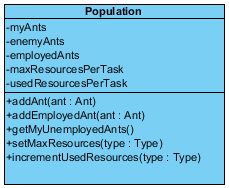
\includegraphics[width=0.5\textwidth]{91_bilder/population}
\caption{Population Klasse}
\label{fig:populationClass}
\end{figure}

Abbildung \ref{fig:populationClass} zeigt unsere Population-Klasse (s. Kapitel \ref{sec:module.Ants.State}), die als zentrale Verwaltungsinstanz f�r unsere Ameisen auch daf�r zust�ndig ist, die allozierten Ressourcen zu verwalten und beim Zuweisen einer Ameise zu einer Aufgabe sicherzustellen, dass das Kontingent nicht �berschritten wird. 

Mit den beiden Feldern \texttt{maxResourcesPerTask} und \texttt{usedResourcesPerTask} wird hier Buch gef�hrt dar�ber, welche Aufgabe wie viele Ameisen verwenden darf, und wie viele sie bereits verwendet hat. Die Aufteilung der Ressourcen, also das Initialisieren von \texttt{maxResourcesPerTask}, geschieht in unserem ResourceAllocator.

\begin{figure}[H]
\centering
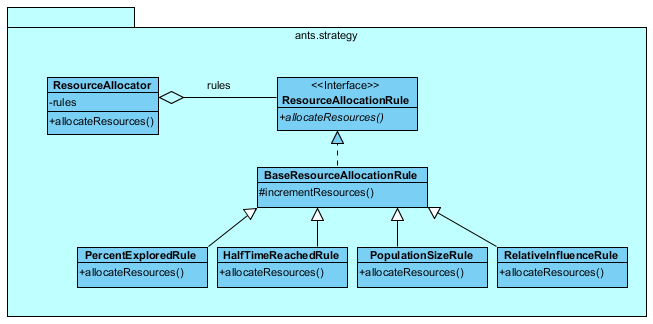
\includegraphics[width=0.9\textwidth]{91_bilder/antsStrategy}
\caption{RessourcenManagement}
\label{fig:antsStrategy}
\end{figure}
 
Abbildung \ref{fig:antsStrategy} zeigt die Klassenhierarchie unserer Ressourcenverwaltung. Die zentrale Klasse ist der ResourceAllocator; mit dessen Methode allocateResources() werden jeweils die Ressourcen neu verteilt:
\lstset{language=Java, tabsize=4}
\begin{lstlisting}
new ResourceAllocator().allocateResources();
\end{lstlisting}
Diese Ressourcenzuteilung wird von unserem Bot jeweils zu Beginn des Zugs vorgenommen. Dazu stellt er als erstes die allozierten Ressourcen pro Aufgabe auf einen definierten Standardwert zur�ck. Diese Werte k�nnen �ber Profile (Kap. \ref{sec:module.Profile}) konfiguriert werden. Dann werden der Reihe nach die konfigurierten Regeln aufgerufen, die jeweils nach ihrer eigenen Logik die Ressourcen f�r bestimmte Aufgaben erh�hen oder verringern. Am Ende entsteht so eine dynamische Ressourcenverteilung, die den verschiedensten Gesichtspunkten Rechnung tragen kann.

\subsection{Implementierte Regeln}
\label{sec:module.resourceMgmt.Regeln}
Wir haben 4 verschiedene Regeln implementiert, die alle von einer gemeinsamen Basisklasse ableiten. Die Basisklasse \texttt{BaseResourceAllocationRule} stellt die Methode \texttt{incrementResources(Type taskType, int increment, Type... tasksToDecrement)} zur Verf�gung, die ein gegebenes Inkrement (Ressourcen-Plus) f�r eine Aufgabe mit gleichm�ssig verteilten Dekrementen (Ressourcen-Minus) auf die angegebenen anderen Aufgaben ausgleicht.

Unsere implementierten Regeln sind:
\begin{itemize}
	\item \textbf{HalfTimeReachedRule:}	Nach Erreichen der Halbzeit des Spiels sorgt diese Regel daf�r, dass das Angreifen der gegnerischen H�gel h�her priorisiert wird.
	\item \textbf{PercentExploredRule:} Diese Regel sorgt daf�r, dass das Erkunden der Umgebung forciert wird, solange nicht ein gewisser Prozentsatz der Karte bereits erforscht ist.
	\item \textbf{PopulationSizeRule:} Diese Regel forciert die Nahrungsbeschaffung; je nach Gr�sse unseres Ameisenvolks tut sie dies st�rker oder weniger stark.
	\item \textbf{RelativeInfluenceRule:} Fall wir eine dominante Position auf dem Spielfeld haben, sorgt diese Regel f�r zus�tzliche Ressourcen f�r die Erkundung (um das Spielfeld weiter zu kontrollieren) und den Angriff auf gegnerische H�gel.
\end{itemize}
All diese Regeln sind �ber Profile konfigurierbar.

Diese Regeln sind nat�rlich nur eine Auswahl dessen, was mit dieser regelbasierten Ressourcenverwaltung m�glich w�re. Viele weitere Regeln w�ren denkbar, aber wir haben in unseren Tests bereits mit diesen vier einfachen Regeln durchaus zufriedenstellende Ergebnisse erzielt. Eine Schwierigkeit bei der Implementierung neuer Regeln gilt es noch zu beachten: Durch die grosse Dynamik des Systems sind die Auswirkungen einer \"Anderung manchmal nur schwer abzusch�tzen; dieser Effekt wird durch die Konfigurierbarkeit des Systems noch verst�rkt. Die Berechenbarkeit des Verhaltens unseres Bots ist also gr�sser, wenn nicht allzu viele Regeln in die Ressourcenverwaltung eingebunden werden.

%L DONE
\section{Profile}
\label{sec:module.Profile}
\"Uber die Profile l�sst sich das Verhalten unseres Bots konfigurativ beeinflussen. Folgende Parameter stehen dazu zur Verf�gung:
\begin{itemize}
\item
\textbf{defaultAllocation.gatherFood}: Standard Ressourcenzuteilung in Prozent f�r die Nahrungssuche. Dieser Wert dient als Startwert f�r den ResourceAllocator.
\item
\textbf{defaultAllocation.explore}:Standard Ressourcenzuteilung in Prozent f�r die Erkundung der Spielwelt. Dieser Wert dient als Startwert f�r den ResourceAllocator.
\item
\textbf{defaultAllocation.attackHills}:Standard Ressourcenzuteilung in Prozent f�r den Angriff auf gegnerische H�gel. Dieser Wert dient als Startwert f�r den ResourceAllocator.
\item
\textbf{defaultAllocation.defendHills}:Standard Ressourcenzuteilung in Prozent f�r die Verteidigung der eigenen H�gel. Dieser Wert dient als Startwert f�r den ResourceAllocator.
\item
\textbf{defendHills.startTurn}: In der Anfangsphase des Spiels macht es nicht viel Sinn, Verteidiger zur�ckzubehalten obwohl kein Angreifer in der N�he ist. Mit diesem Parameter kann eingestellt werden, ab welchem Zug wir pro H�gel mindestens einen Verteidiger abkommandieren.
\item
\textbf{defendHills.minControlRadius}: Dieser Parameter legt fest, wie gross das Gebiet um unsere H�gel ist, das wir verteidigen.
\item
\textbf{explore.forceThresholdPercent}: Schwellenwert f�r das Verh�ltnis von nie gesehenen Zellen zu allen Zellen auf der Karte. Wenn der Wert unter diesem Schwellenwert liegt, werden zus�tzliche Ressourcen f�r die Erkundung bereitgestellt.
\item
\textbf{explore.forceGain}: Dieser Wert bestimmt, um wie viel die Ressourcen f�r die Erkundung erh�ht werden, falls obiger Schwellenwert unterboten wird. M�gliche Werte liegen zwischen 0 und 1.
\item
\textbf{explore.dominantPositionBoost}: Wenn wir eine dominante Position auf dem Spielfeld haben, wird die Erkundung gest�rkt, um die Karte zu kontrollieren. Dieser Parameter bestimmt, wie viel zus�tzliche Ressourcen zugeteilt werden.
\item
\textbf{attackHills.dominantPositionBoost}: Wenn wir eine dominante Position auf dem Spielfeld haben, wird der Angriff auf gegnerische H�gel forciert, um Punkte zu sammeln. Dieser Parameter bestimmt, wie viel zus�tzliche Ressourcen zugeteilt werden.
\item
\textbf{attackHills.halfTimeBoost}: Nach Ablauf der H�lfte der Spielzeit erh�hen wir die Aggressivit�t unseres Bots. Dieser Parameter bestimmt, wie stark der Angriff auf gegnerische H�gel in der 2. Halbzeit forciert wird.
\end{itemize}

\subsection{Validierung}
\label{sec:module.Profile.Validierung}
Die Parameter \texttt{defaultAllocation.*} m�ssen in der Summe 100 ergeben. Dies wird beim Start des Bots, wenn das Profil geladen wird, �berpr�ft. Auch f�r die anderen Parameter sind Validierungen vorhanden (z.B. Pr�fung, ob ein Prozentwert zwischen 0 und 100 liegt.)

Fehlt ein Parameter in einem Profil, so wird f�r diesen Parameter der Standardwert genommen.

\subsection{Definierte Profile}
\label{sec:module.Profile.DefinierteProfile}
Folgende Profile sind im Bot definiert und k�nnen beim Start ausgew�hlt werden:

\renewcommand{\arraystretch}{1.5}
		\begin{tabular}{ l | r | r | r | r }
			Parameter & Default & Aggressive & Defensive & Expansive \\
			\hline
			defaultAllocation.gatherFood & 25 & 20 & 25 & 30\\
			defaultAllocation.explore & 25 & 20 & 25 & 30\\
			defaultAllocation.attackHills & 25 & 45 & 15 & 20\\
			defaultAllocation.defendHills & 25 & 15 & 35 & 20\\
			defendHills.startTurn & 30 & 30 & 20 & 30\\
			defendHills.minControlRadius & 8 & 8 & 12 & 8\\
			explore.forceThresholdPercent & 80 & 80 & 80 & 90\\
			explore.forceGain & 0.25 & 0.25 & 0.25 & 0.4\\
			explore.dominantPositionBoost & 5 & 5 & 5 & 8\\
			attackHills.dominantPositionBoost & 2 & 5 & 2 & 2\\
			attackHills.halfTimeBoost & 20 & 25 & 15 & 20\\
		\end{tabular}



\subsection{Weiterentwicklungs-Potenzial}
\label{sec:module.Profile.Weiterentwicklung}
Aktuell k�nnen 11 Parameter via Profil angepasst werden, wovon die meisten einen Einfluss auf das Ressourcen-Management haben. Weitere Parameter f�r beliebige Teile der Logik k�nnten problemlos eingef�gt werden und m�ssten sich auch nicht auf numerische Werte beschr�nken. Denkbar w�ren bspw. ganze Strategien, die per Profil einfach ausgetauscht werden k�nnten.%L DONE OK
\chapter{Logging}
\label{sec:module.Logging}

Nach einem absolvierten Spiel analysierten wir jeweils die Spielsituationen, welche sich ergeben haben. Dazu geh�rte das Analysieren des geschriebenen Logs. Dabei bedienten wir uns den nachfolgenden Mechanismen.

\section{Logkategorien und Loglevel}
\label{sec:module.Logging.LogkategorienundLoglevel}

Jeder Logeintrag geh�rt einer Logkategorie an. Je Logkategorie kann der Loglevel defniert werden. Die Loglevel lauten TRACE, DEBUG, INFO und ERROR. Wenn also zum Beispiel bei der Logkategorie ATTACKHILLMISSION der Loglevel auf INFO gestellt ist, werden nur die Fehler auf Stufe INFO und ERROR in das Logfile geschieben. Zudem kann, falls erw�nscht, jede Logkategorie in ein eigenes Logfile geschrieben werden. Die meisten Module habe ihre eigene Logkategorie, so kann durch korrekte Logeinstellung erzwungen werden dass nur die Logs, welche f�r das Analysieren eines bestimmten Spielmoduls von Bedeutung sind, ins Logfile geschrieben werden. Dadurch m�ssen nicht riesige Mengen an Logs druchw�lzt werden um an die Informationen heran zu kommen.


\section{JavaScript Addon f�r HMTL-Gameviewer}
\label{sec:module.Logging.Addon}
Das Codepaket welches von den Challenge-Organisatoren mitgeliefert wird, bietet bereits eine hilfreiche 2D-Visualisierung des Spiels, mit welchem das Spielgeschehen mitverfolgt werden kann. Die Visualisierung wurde mit HMTL und Javascript implementiert. Leider ist es nicht m�glich zus�tzliche Informationen auf die Seite zu projizieren. Deshalb haben wir den Viewer bereits im Projekt 2 mit einer solchen Funktion erweitert. Mit der Codezeile Logger.liveInfo(...) kann eine Zusatzinformation geschrieben werden, welche auf dem Viewer sp�ter sichtbar ist. Es muss definiert werden mit welchem Zug und wo auf dem Spielfeld die Infomation angezeigt werden soll. Im Beispiel wird an der Position der Ameise (ant.getTile()) ausgegeben welchen Task die Ameise hat.
\begin{verbatim}
Logger.liveInfo(Ants.getAnts().getTurn(), ant.getTile(), 
                "Task: %s ant: %s", issuer, ant.getTile());
\end{verbatim}
Auf der Karte wird ein einfaches aber praktisches Popup mit den geschriebenen Informationen angezeigt. Dank solcher Zusatzinformationen muss nicht m�hsam im Log nachgeschaut werden, welcher Ameise wann und wo welcher Task zugeordnet ist.

\begin{figure}[H]
\centering
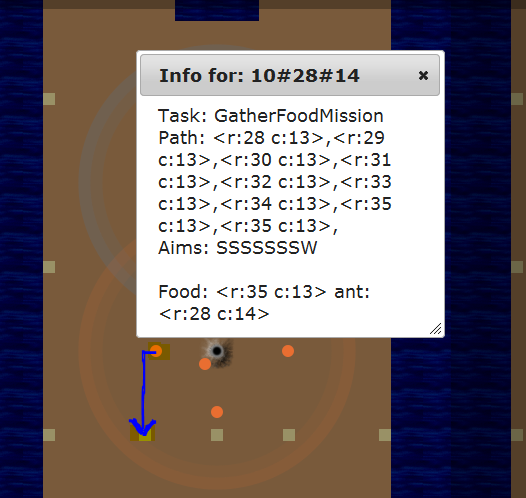
\includegraphics[height=70mm]{91_bilder/javascriptAddon.png}
\label{fig.javascriptAddon}
\caption[Live-Info Popupfenster]{Im Popupfenster steht die Aufgabe der Ameise sowie die Pixel des Pfades (falls vorhanden), welcher die Ameise ablaufen wird.}
\end{figure}

Das angezeigte Popup zeigt welchen Task (GatherFoodTask) die Ameise hat, wo sie sich befindet <r:28 c:14>, welches Futterpixel angesteuert wird <r:35 c:13> und welchen Pfad dazu berechnet wurde. Im Rahmen der Bachelorarbeit wurde dieses Addon erweitert. Nun werden alle Pixel welche in dem Popup ausgegeben werden auf der Karte markiert. Siehe (Abb. \ref{fig.javascriptAddon2})

\begin{figure}[H]
\centering
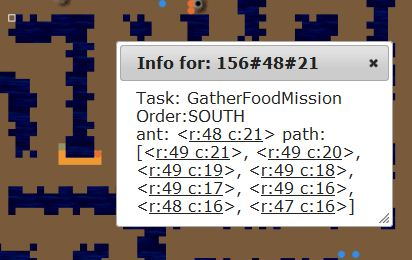
\includegraphics[height=45mm]{91_bilder/javascriptAddon2.jpg}
\label{fig.javascriptAddon2}
\caption[Erweiterung des Live-Info Popupfenster]{Mit der erweiterten Version wird der Pfad (orange) der Ameise von <r:48 c:21> nach <r:47 c:16> auf der Karte abgebildet.}
\end{figure}%L DONE OK

\chapter{Testing}
\label{chap:testing} 

Dieses Kapitel beschreibt, wie wir unseren Bot und dessen Komponenten getestet haben. Das Testen beanspruchte einen grossen Teil unserer aufgewendeten Zeit. Die nachfolgenden Methoden zeigen auf, wie wir versuchten m�glichst effizient zu testen, so dass uns mehr Zeit f�r das implementieren der Module blieb. In vielen F�llen machten wir gute Erfahrungen damit, mit gezielten Unit-Tests die Entwicklung des Codes voranzutreiben. Zu behaupten, wir h�tten dabei Test Driven Development (TDD)\footnote{Bei der testgetriebenen Entwicklung erstellt der Programmierer Software-Tests konsequent vor den zu testenden Komponenten. (Def. Wikipedia)} angewandt, w�re �bertrieben, aber bei verschiedenen Modulen orientierten wir uns an den Ideen von TDD, um rasch und zuverl�ssig funktionierende Code zu schreiben.

\section{UnitTests}
\label{sec:testCenter.UnitTests}

Dank dem modularen Aufbau des Java-Codes war es uns gut m�glich, einzelne Module zu testen. F�r unsere UnitTests verwendeten wir die JUnit 4 Library. So findet man in jedem Java Project das Code-Package und ein UnitTest-Package, welches den Code auf dessen Richtigkeit pr�ft. Die Module wurden erst nach den erfolgreichen UnitTests in den Bot eingebaut. Dies hat den Vorteil, dass die Fehlern nicht im laufenden Spiel auftraten und wir die Ursachen  m�hsam suchen mussten.

Beim Combat Positioning\footnote{siehe Kapitel \ref{sec:module.CombatSituation}} haben wir uns am meisten an Test Driven Development orientiert. Wir haben im Test verschiedenste Szenarien eingegeben, die im Kampf auftauchen k�nnten, und haben dann den Code so erweitert, dass f�r diese Szenarien gute L�sungen gefunden wurden. Auf diese Weise sind wir bei der jetzigen Implementierung des Combat Positioning angekommen, die eine ganz gute N�herung an eine optimale Kampfformation darstellt.

\section{Visuelle Tests}
\label{sec:testCenter.VisuelleTests}

In Form eines UnitTest haben wir auch unsere visuellen Tests geschrieben. Eine visuelle �berpr�fung des Resultats ist meistens, vor allem bei der Pfadsuche, einfacher zu kontrollieren. Im Gegensatz zu JUnit wo das zu erwartende Resultat mit Assertions (z.B. \texttt{assertEquals()}) gepr�ft wird, haben die visuellen Test ein HTML-File als Output. In das HTML-File wird die Karte in Tabellenform gespeichert. In jeder Zelle der Tabelle k�nnen Objekte (Einheiten, H�gel, Wegpunkte etc.) durch farbige Punkte dargestellt werden. Diese Funktionalit�ten bietet die extra daf�r geschriebene Klasse MapOutput. Nachfolgend ist ein HTML-File abgebildet mit welchem wir die Korrektheit des Clustering und des HPA* Algorithmus visuell �berpr�ft haben. 

\begin{figure}[H]
\centering
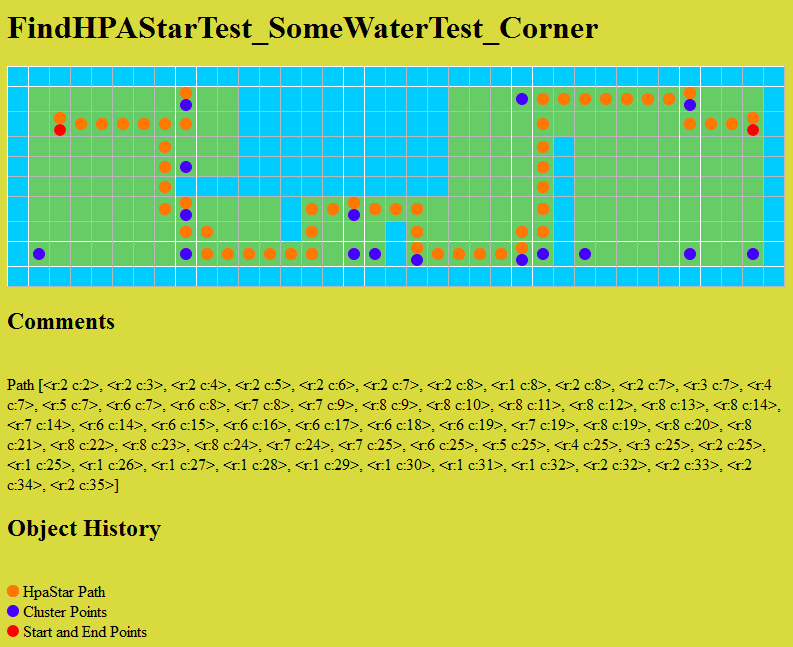
\includegraphics[height=100mm]{91_bilder/mapoutput01}
\caption{HTML-Ausgabe zur visuellen �berpr�fung von HPA*}
\label{fig:mapoutput01}
\end{figure}%S DONE OK
\section{Testbots}
\label{sec:testCenter.Testbots}

Eine weitere Testmethode war, Testbots zu erstellen. Zum Beispiel haben wir den DefendHillBot erstellt. Dieser hat die Eigenschaft, nur zu verteidigen, nicht aber anzugreifen. Wir nahmen eine kleine Karte, so dass es schnell zu Angriffen des Gegners kam. Dadurch konnten wir unser Verteidigungvserhalten nach nur kurzer Spieldauer genau analysieren und verbessern.

Dasselbe galt f�r den AttackHillBot. Wir haben wiederum eine kleine Karte genommen auf der viel Futter vorhanden ist, so dass sich das Ameisenvolk schnell vermehrt. Dank der beschr�nkten Karte kam es schnell zu Angriffen, und wir konnten so unsere Berechnung der  Angriffsformationen testen.

Im Kapitel Task wurde beschrieben, welche Task bzw. Missionen nicht erfolgversprechend waren und wir nicht weiterverfolgt haben. Bevor wir das aber wussten, haben wir, um die Funktionen zu testen, wiederum einen speziellen Bot erstellt. Anhand der Ergebnisse konnten wir herausfinden, dass diese Methoden nicht praktikabel waren und wir die Ideen verworfen haben. So sind im Code noch folgende Bots zu finden:
\begin{itemize}
	\item ConcentrateBot
	\item FlockBot
	\item SwarmBot		
\end{itemize}
F�r diese Bots sind zwar noch ANT-Targets\footnote{s. Kapitel \ref{chap:spielanleitung.Ausfuehrung}} zum Ausf�hren der Tests vorhanden, da die Bots aber, nachdem sie ihren Zweck erf�llt hatten, nicht mehr weiterentwickelt wurden, lassen sich mit den meisten Bots keine Spiele mehr starten.



%S DONE OK
\section{Performance Suchalgorithmen}
\label{sec:testCenter.PerformanceSuchalgorithmen}

Die entwickelten Suchstrategien werden in diesem Kapitel verglichen. Zum Vergleich wird eine Testkarte der Gr�sse 100 x 110 Tiles verwendet, auf dieser werden die Pfadsuchalgorithmen angewendet. Die Suchstrategie \texttt{SIMPLE} wird nicht in den Vergleich einbezogen, diese ist wie beschrieben nur f�r kurze Pfade einsetzbar. Daf�r wird der HPA* mit zwei verschiedenen Clustergr�ssen (14 \& 20), sowie den unterschiedlichen Typen \texttt{Corner} und \texttt{Centered} angewendet. Der erste Test beinhaltet zwei Durchg�nge, bei welchen jeweils ein anderer Start- und Zielort definiert wurde.

\begin{table}[H]
	%weird hack to enable footnotes in the table
	\begin{minipage}{20cm}

		\begin{tabular}{ l | r  r  | r  r | r r }
		
		&  \multicolumn{2}{l|}{\textbf{1. Durchlauf}} & \multicolumn{2}{l|}{\textbf{2. Durchlauf}} &
		\multicolumn{2}{l}{\textbf{Durchschnitt}} \\
		
		\textbf{Suchalgorithmus} & \textbf{Dauer\footnote{Dauer in Millisekunden}} & \textbf{Pfadl�nge\footnote{Pfadl�nge in Anzahl Tiles}} & \textbf{Dauer} &
		\textbf{Pfadl�nge} & \textbf{Dauer} & \textbf{Pfadl�nge}  \\
		\hline
		
		A* & 124.6 & 95 & 101.2 & 95 & 112.9 &	95 \\
		HPA* (Centered,14)\footnote{Typ: Centered, Clustergr�sse: 14} & 167.6 & 99 & 25.2 & 107 & 96.4 & 103\\
		HPA* (Corner,14) & 2677.4 & 117 & 2394.6 & 117 & 2536 & 117 \\
		HPA* (Centered,20)  & 6.4 & 106 & 60 & 137 & 33.2 & 121.5 \\
		HPA* (Corner,20) & 22 & 113 & 231 & 133 & 126.5 & 123 \\
		\end{tabular}\par
		\vspace{-0.75\skip\footins}
   \renewcommand{\footnoterule}{}
  \end{minipage}
	\caption{Testresultate: Vergleich der Suchalgorithmen}
	\label{tab:testSearchAlgorithms}
\end{table}



In der Tabelle \ref{tab:testSearchAlgorithms} sind die Testresultate aufgelistet. Zu sehen ist, dass nur A* den optimalen Pfad von 95 \gls{Tile}s findet, und zwar in ca. 120 Millisekunden. HPA* mit Typ \texttt{Corner} und mit der kleinerer Clustergr�sse von 14 \gls{Tile}s ist langsamer als A*. Dies ist darauf zur�ckzuf�hren, dass mit dieser Einstellung das Clusternetz von HPA* zu feinmaschig ist. Um den Pfad zu finden m�ssen viele Kanten und Knoten der geclusterten Karte durchforscht werden. Das dauert l�nger als bei A*, wo die Nachfolgerknoten einfach aus einem zweidimensionalen Array gelesen werden.

Der Typ \texttt{Centered} ist deutlich schneller als der Typ \texttt{Corner}, da er in etwa nur halb so viele Pfadknoten pr�fen muss (siehe Kapitel \ref{subsec:module.Suchalgorithmen.Pfadsuche.HPAstar}). Sobald die Clustergr�sse auf 20 \gls{Tile}s gestellt wird, ist HPA* deutlich schneller als A*. Allgemein muss aber gesagt werden, dass es sehr darauf an kommt, ob die Gel�ndestruktur dem Clustering entgegenkommt, so dass die Verbindungspunkte g�nstig gelegen sind und ein Pfad gefunden werden kann der nicht zu viele Umwege macht. Abbildung \ref{fig:comapreSearchStrategies} zeigt, wie die verschiedenen Suchalgorithmen den Pfad zwischen den zwei schwarzen Punkten gefunden haben.

\begin{figure}[H]
\centering
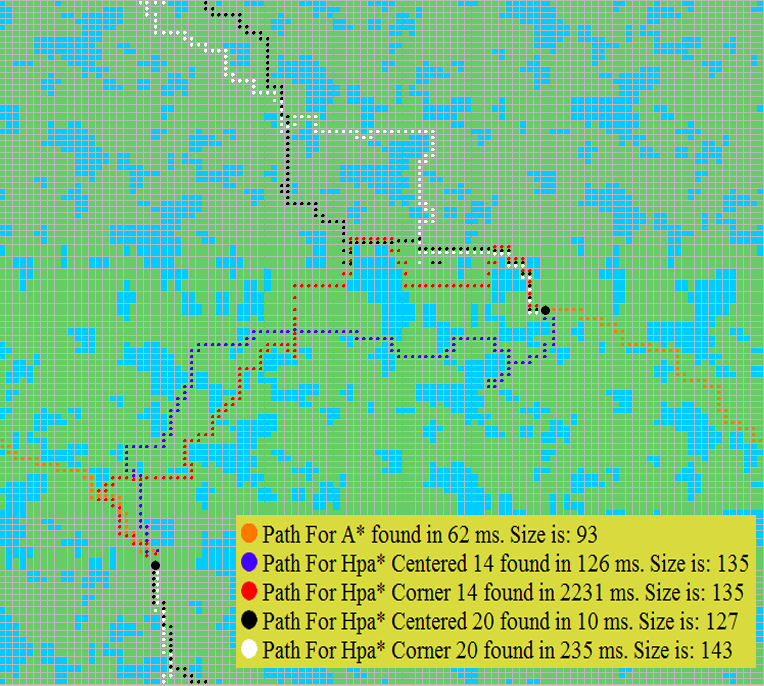
\includegraphics[height=100mm]{91_bilder/searchcompare}
\caption[Vergleich der Suchalgorithmen]{Vergleich der gefundenen Pfade: Viele Wege f�hren nach Rom.}
\label{fig:comapreSearchStrategies}
\end{figure}

Beim ersten Test wurde der Pfad nicht gesmoothed, und auch die Zeit, welche es brauchte um die Karte in Cluster aufzuteilen, ist nicht ber�cksichtigt. Nachfolgender Test ber�cksichtigt nun diese zwei Aspekte.

\begin{table}[H]
	%weird hack to enable footnotes in the table
	\begin{minipage}{11cm}

		\begin{tabular}{ l | r r r r r }
		
		\textbf{Suchalgorithmus} & \textbf{Clustering} & \textbf{Pfadsuche} & \textbf{PathSmoothing} & 
		\textbf{Pfadl�nge 1}\footnote{ohne Smoothing} & \textbf{Pfadl�nge 2}\footnote{mit Smoothing}  \\
		\hline		
		A* & - & 95 ms & - & 95 & -  \\
		HPA* (Centered,20)  & 484 ms & 4 ms & 16 ms & 127 & 119 \\
		\end{tabular}\par
		\vspace{-0.75\skip\footins}
   \renewcommand{\footnoterule}{}
  \end{minipage}
	\caption[Testresultate: Vergleich der Suchalgorithmen mit PathSmoothing]{Testresultate: Dauer, mit Ber�cksichtigung von Clustering und PathSmoothing}
	\label{tab:totalDuration}
\end{table}

Um die Cluster f�r die ganze Karte zu berechnen braucht es einmalig ungef�hr 480 Millisekunden. Weil in einem konkreten Spiel die Karte nur nach und nach erkundet wird, verteilt sich der Aufwand f�r das Clustering auf mehrere Z�ge und ist deswegen f�r uns nicht kritisch. Wenn wir einen gegl�tteten HPA* wollen, brauchen wir ca. 20 ms pro Suche; f�r den optimalen Pfad mit A* 95 ms. Mit Verwendung von HPA*, sparen wir im Schnitt rund 70 ms pro Pfadsuche. Wenn man ber�cksichtigt, dass pro Zug f�r mehrere Ameisen ein Pfad gesucht wird, lohnt sich der Einsatz von HPA* allemal.%S DONE OK
\section{Testreport Profile}
\label{sec:testCenter.TestreportProfile}
 
Um die verschiedenen Profile unseres Bots zu testen, f�hrten wir diverse Testl�ufe durch, in denen wir die verschieden konfigurierten Bots jeweils 100 Mal gegen verschiedene Gegner und gegeneinander antreten liessen. F�r diese Testl�ufe wurden die in Tabelle \ref{tab:definierteProfile} aufgef�hrten Profile verwendet.

W�hrend der Entwicklung f�hrten wir die meisten Tests gegen den Bot von Evan Greavette (Username egreavette) durch. Er hatte seinen Bot �ber GitHub ver�ffentlicht: \url{https://github.com/egreavette/Ants-AI}. Daher f�hrten wir auch die ersten Testl�ufe gegen diesen Gegner durch:

\renewcommand{\arraystretch}{1.5}
\begin{table}[H]
	\centering
		\begin{tabular}{ l | r  r  r  r }
			\textbf{Profil} & \textbf{Siege} & \textbf{Unentschieden} & \textbf{Niederlagen} & \textbf{Total Punkte} \\
			\hline
			Default & 62 & 13 & 25 & 957:579\\
			Aggressive & 61 & 18 & 21 & 1005:642\\
			Defensive & 53 & 15 & 32 & 915:726\\
			Expansive & 59 & 16 & 25 & 955:673
		\end{tabular}
	\caption{Bilanz der Testl�ufe gegen egreavette}
	\label{tab:testAgainstEgreavette}
\end{table}

Wie man unschwer erkennen kann, sind gegen diesen Gegner drei der Profile ungef�hr gleichwertig; lediglich der Defensive Bot f�llt etwas ab.

Als n�chstes f�hrten wir einen Testlauf gegen den Sieger des Wettbewerbs durch. Mathis Lichtenberger (Username xathis) hatte seinen Bot ebenfalls �ber GitHub zur Verf�gung gestellt: \url{https://github.com/xathis/AI-Challenge-2011-bot}. 

\begin{table}[H]
	\centering
		\begin{tabular}{ l | r  r  r  r }
			\textbf{Profil} & \textbf{Siege} & \textbf{Unentschieden} & \textbf{Niederlagen} & \textbf{Total Punkte} \\
			\hline
			Default & 17 & 7 & 76 & 521:1094\\
			Aggressive & 23 & 11 & 66 & 593:1010\\
			Defensive & 11 & 8 & 81 & 479:1106\\
			Expansive & 24 & 6 & 70 & 610:988
		\end{tabular}
	\caption{Bilanz der Testl�ufe gegen xathis}
	\label{tab:testAgainstXathis}
\end{table}

Gegen diesen starken Gegner zeigen sich bereits deutlichere Unterschiede zwischen den Profilen. Man sieht, dass die beiden offensiver ausgerichteten Profile (Aggressive und Expansive) sich deutlich besser schlagen, w�hrend das Defensive Profil deutlich abf�llt. Dies entspricht in etwa unseren Erwartungen. Die St�rken von xathis' Bot liegen eindeutig in der Offensive, w�hrend die Defensive nicht das Prunkst�ck unseres Bots ist. Deshalb k�nnen wir in der Verteidigung gegen xathis fast nur verlieren und haben eine gr�ssere Chance, wenn wir selber in die Offensive gehen.

Als n�chstes liessen wir unsere 4 Profile gegeneinander antreten:

\begin{table}[H]
	\centering
		\begin{tabular}{ l | r  r  r  r }
			\textbf{Profil} & \textbf{Siege} & \textbf{Unentschieden} & \textbf{Niederlagen} & \textbf{Total Punkte} \\
			\hline
			Default & 22 & 7 & 71 & 332:891\\
			Aggressive & 23 & 10 & 67 & 314:909\\
			Defensive & 23 & 8 & 69 & 300:923\\
			Expansive & 16 & 7 & 77 & 277:946
		\end{tabular}
	\caption{Bilanz der Testl�ufe gegeneinander}
	\label{tab:test4Profile}
\end{table}

Hier zeigt sich, dass die Profile im Kampf gegeneinander relativ ausgeglichen sind. Es zeigt sich auch, dass das expansive Verhalten sich gegen mehrere Gegner weniger lohnt, da sich dabei die Ameisen eher auf dem Spielfeld verzetteln und man Gefahr l�uft, isolierte Ameisen zu verlieren.

Alles in allem waren aber diese Standard-Profile noch mehr oder weniger gleichwertig. Wir erstellten daher neue, st�rker vom Standard abweichende Profile und f�hrten noch einmal Testl�ufe gegen xathis und gegeineinander durch.

\renewcommand{\arraystretch}{1.5}
\begin{table}[H]
	\centering
		\begin{tabular}{ l | r  r  r  r }
			\textbf{Parameter} & \textbf{Default} & \textbf{Aggressive 2} & \textbf{Defensive 2} & \textbf{Expansive 2}\\
			\hline
			defaultAllocation.gatherFood & 25 & 15 & 25 & 35\\
			defaultAllocation.explore & 25 & 15 & 25 & 35\\
			defaultAllocation.attackHills & 25 & 60 & 10 & 20\\
			defaultAllocation.defendHills & 25 & 10 & 40 & 10\\
			defendHills.startTurn & 30 & 30 & 20 & 50\\
			defendHills.minControlRadius & 8 & 8 & 20 & 8\\
			explore.forceThresholdPercent & 80 & 80 & 80 & 90\\
			explore.forceGain & 0.25 & 0.1 & 0.25 & 0.4\\
			explore.dominantPositionBoost & 5 & 3 & 5 & 10\\
			attackHills.dominantPositionBoost & 2 & 10 & 2 & 2\\
			attackHills.halfTimeBoost & 20 & 40 & 15 & 20\\
		\end{tabular}
		\caption{Die Profile f�r den 2. Testlauf}
		\label{tab:definierteProfile2}
\end{table}

\begin{table}[H]
	\centering
	%weird hack to enable footnotes in the table
	\begin{minipage}{11cm}
    \centering
		\begin{tabular}{ l | r  r  r  r }
			\textbf{Profil} & \textbf{Siege} & \textbf{Unentschieden} & \textbf{Niederlagen} & \textbf{Total Punkte} \\
			\hline
			Default & 17 & 7 & 76 & 521:1094\footnote{Da sich an diesem Profil nichts ge�ndert hatte, wurde der Testlauf nicht noch einmal durchgef�hrt; die Werte stammen aus dem 1. Lauf}\\
			Aggressive & 20 & 4 & 76 & 545:1040\\
			Defensive & 13 & 4 & 83 & 385:1186\\
			Expansive & 19 & 12 & 69 & 578:1010
		\end{tabular}\par
		\vspace{-0.75\skip\footins}
   \renewcommand{\footnoterule}{}
  \end{minipage}
	\caption{Bilanz der 2. Testl�ufe gegen xathis}
	\label{tab:testAgainstXathis2}
\end{table}

Aus Tabelle \ref{tab:testAgainstXathis2} sieht man, dass die neuen Profile gegen xathis eher schlechter abschnitten, aber die Unterschiede zum 1. Testlauf sind nur gering.

\begin{table}[H]
	\centering
		\begin{tabular}{ l | r  r  r  r }
			\textbf{Profil} & \textbf{Siege} & \textbf{Unentschieden} & \textbf{Niederlagen} & \textbf{Total Punkte} \\
			\hline
			Default & 41 & 9 & 50 & 428:788\\
			Aggressive & 12 & 7 & 81 & 276:940\\
			Defensive & 22 & 6 & 72 & 256:960\\
			Expansive & 11 & 10 & 79 & 256:960
		\end{tabular}
	\caption{Bilanz der 2. Testl�ufe gegeneinander}
	\label{tab:test4Profile2}
\end{table}

Wie Tabelle \ref{tab:test4Profile2} zeigt, waren die Unterschiede zwischen den neuen Profilen im Kampf gegeneinander schon deutlich sichtbarer. Die extremeren Profile weisen alle eine deutlich schlechtere Bilanz auf, wobei die Defensive Konfiguration noch am besten f�hrt. Gegen diese Profile ist unsere ausgewogene Standardkonfiguration aber bereits ein deutlicher Sieger.

\subsection{TestReader}
\label{sec:module.Testreader}
F�r die Auswertung der Testl�ufe haben wir ein kleines Zusatzmodul geschrieben, das aus den Spielberichten der Spielengine die relevanten Informationen auslesen kann. Es besteht lediglich aus einer einzelnen Klasse (\texttt{TestReader} mit einer main() Methode. Es liest aus dem Log-Verzeichnis die *.replay Dateien (Spielberichte im Json-Format) ein, parsed sie mit Hilfe der Simple-Json Bibliothek und erstellt eine CSV-Datei mit den wichtigsten Ergebnissen aus den einzelnen Spielen. Ausserdem wird eine zus�tzlich CSV-Datei ausgegeben, die die Ergebnisse aggregiert, und zwar ungef�hr in der Form, wie sie in diesem Kapitel in den Tabellen ersichtlich ist.%L DONE OK
\section{Online Tests}
\label{sec:testCenter.Online}
Anfangs Dezember stellten wir fest, dass ein User aus dem alten AI-Challenge Forum mit dem Namen ''smiley1983`` einen TCP-Server aufgesetzt hatte, �ber welchen man Bots gegeneinander antreten lassen konnte. Nat�rlich probierten wir das aus und f�hrten auch um die 50 Spiele �ber diesen Server aus. F�r aussagekr�ftige Tests war die Teilnehmerzahl auf diesem Server aber zu gering, weshalb wir uns dagegen entschieden, diese Option in unser Testkonzept aufzunehmen.%L DONE OK

\chapter{Spielanleitung}
\label{chap:spielanleitung}

\section{Systemvoraussetzungen}
\label{chap:spielanleitung.voraussetzungen}

Um ein Spiel ausf�hren zu k�nnen, muss auf dem Computer folgende Software installiert sein:
\begin{enumerate}
\item Java SE JDK Version 6 \footnote{\url{http://www.oracle.com/technetwork/java/javasebusiness/downloads/java-archive-downloads-javase6-419409.html}}
\item Python \footnote{\url{http://www.python.org/download/}}
\item ANT \footnote{\url{http://ant.apache.org/bindownload.cgi}}
\end{enumerate}

Falls das Spiel mit anderen als den vorkonfigurierten Gegnern gestartet werden soll, muss evtl. noch andere Software installiert werden, je nachdem in welcher Programmiersprache die entsprechenden Bots geschrieben sind.

\section{Ausf�hren eines Spiels}
\label{chap:spielanleitung.Ausfuehrung}
  
Im Ordner \texttt{Code} befinden sich unsere Eclipse-Projekte mit dem gesamten Source-Code unserer Implementation, und der offiziellen Spiel-Engine. Das Hauptprojekt befindet sich im Unterordner \texttt{Ants}. Zum einfachen Ausf\"uhren eines Spiels haben wir dort ein ANT-Buildfile (build.xml) erstellt. Dieses definiert verschiedene Targets, mit denen ein Spiel mit jeweils unterschiedlichen Parametern gestartet werden kann.
Falls ANT korrekt installiert ist, k�nnen diese Targets aus dem \texttt{Ants}-Verzeichnis heraus einfach mit ''\texttt{ant <targetName>}`` aufgerufen werden. 
\begin{enumerate}
\item
Das Target \texttt{testBot} ist lediglich zum einfachen Testen eines Bots sinnvoll und entspricht dem Spiel, das verwendet wird, um Bots, die auf der Website hochgeladen werden, zu testen.
\item
Das Target \texttt{runTutorial} f\"uhrt ein Spiel mit den Parametern aus, die im Tutorial auf der Website zur Erkl\"arung der Spielmechanik verwendet werden.
\item
Die Targets \texttt{mazeAgainst*} f\"uhren jeweils ein Spiel auf einer komplexeren und gr\"osseren, labyrinthartigen Karte aus, und zwar gegen den jeweils bezeichneten Gegner.
\item
Das Target \texttt{maze4Players} f�hrt ein Spiel gegen drei andere Bots auf einer noch etwas gr�sseren Karte durch.
\item
Die Targets \texttt{mazeProfiles} und \texttt{mazeProfiles4Players} sind dazu da, mehrere Kopien unseres Bots mit verschiedenen Profilen gegeneinander antreten zu lassen. Wie im Kapitel \ref{sec:module.Logging.Profile} erw�hnt, muss dazu erst in der Klasse LiveInfo das LiveInfo-Logging deaktiviert werden: 
\lstset{language=Java, tabsize=4}
\begin{lstlisting}
private static boolean enabled = false;
\end{lstlisting}
\item 
Das Target \texttt{testOnline} l�sst den Bot �ber einen privaten TCP-Server gegen andere Bots antreten, unter �hnlichen Bedingungen wie beim eigentlichen Wettbewerb, nur leider mit deutlich weniger Teilnehmern. (s. Kapitel \ref{sec:testCenter.Online})
\item
Die Targets \texttt{repeat*} dienten der Durchf�hrung der Profil-Testl�ufe und sind ansonsten wenig interessant.
\item
Die Targets \texttt{debug*} dienten dem Starten unserer Testbots, die wir w�hrend der Entwicklung einsetzten (s. Kapitel \ref{sec:testCenter.Testbots}).
\end{enumerate}

Bei den meisten dieser Targets erscheint beim Starten eine Abfrage, welches Profil man gerne starten w�rde. Hier stehen die in Kapitel \ref{sec:module.Profile.DefinierteProfile} beschriebenen Profile zur Auswahl.

Im Unterordner \texttt{tools} befindet sich die in Python implementierte Spiel-Engine. Unter \texttt{tools/maps} liegen noch weitere vordefinierte Umgebungen, und unter \texttt{tools/mapgen} liegen verschiedene Map-Generatoren, die zur Erzeugung beliebiger weiterer Karten verwendet werden k\"onnen. 

Im Unterordner \texttt{tools/sample\_bots} befinden sich einige einfache Beispiel-Bots, gegen die man spielen kann. 

Im Unterordner \texttt{tools/bots} haben wir Kopien der Bots von einigen Teilnehmern abgelegt, gegen die wir im Zug der Entwicklung immer wieder getestet haben. %L DONE OK
%todo:
%Glossar
%Bibliographie
%Entscheidungen dokumentieren (warum dieser Algorithmus, warum nicht dieses Design Pattern, ...)
%einheitliche Listings mit caption
%literaturverzeichnisngs 
%Bibliographie: papers influence map , hpa* und pathsmoothing


% Attachment:
%---------------------------------------------------------------------------
%\appendix
%\settocdepth{section}
%\chapter{Spielanleitung}
\label{chap:spielanleitung}

\section{Systemvoraussetzungen}
\label{chap:spielanleitung.voraussetzungen}

Um ein Spiel ausf�hren zu k�nnen, muss auf dem Computer folgende Software installiert sein:
\begin{enumerate}
\item Java SE JDK Version 6 \footnote{\url{http://www.oracle.com/technetwork/java/javasebusiness/downloads/java-archive-downloads-javase6-419409.html}}
\item Python \footnote{\url{http://www.python.org/download/}}
\item ANT \footnote{\url{http://ant.apache.org/bindownload.cgi}}
\end{enumerate}

Falls das Spiel mit anderen als den vorkonfigurierten Gegnern gestartet werden soll, muss evtl. noch andere Software installiert werden, je nachdem in welcher Programmiersprache die entsprechenden Bots geschrieben sind.

\section{Ausf�hren eines Spiels}
\label{chap:spielanleitung.Ausfuehrung}
  
Im Ordner \texttt{Code} befinden sich unsere Eclipse-Projekte mit dem gesamten Source-Code unserer Implementation, und der offiziellen Spiel-Engine. Das Hauptprojekt befindet sich im Unterordner \texttt{Ants}. Zum einfachen Ausf\"uhren eines Spiels haben wir dort ein ANT-Buildfile (build.xml) erstellt. Dieses definiert verschiedene Targets, mit denen ein Spiel mit jeweils unterschiedlichen Parametern gestartet werden kann.
Falls ANT korrekt installiert ist, k�nnen diese Targets aus dem \texttt{Ants}-Verzeichnis heraus einfach mit ''\texttt{ant <targetName>}`` aufgerufen werden. 
\begin{enumerate}
\item
Das Target \texttt{testBot} ist lediglich zum einfachen Testen eines Bots sinnvoll und entspricht dem Spiel, das verwendet wird, um Bots, die auf der Website hochgeladen werden, zu testen.
\item
Das Target \texttt{runTutorial} f\"uhrt ein Spiel mit den Parametern aus, die im Tutorial auf der Website zur Erkl\"arung der Spielmechanik verwendet werden.
\item
Die Targets \texttt{mazeAgainst*} f\"uhren jeweils ein Spiel auf einer komplexeren und gr\"osseren, labyrinthartigen Karte aus, und zwar gegen den jeweils bezeichneten Gegner.
\item
Das Target \texttt{maze4Players} f�hrt ein Spiel gegen drei andere Bots auf einer noch etwas gr�sseren Karte durch.
\item
Die Targets \texttt{mazeProfiles} und \texttt{mazeProfiles4Players} sind dazu da, mehrere Kopien unseres Bots mit verschiedenen Profilen gegeneinander antreten zu lassen. Wie im Kapitel \ref{sec:module.Logging.Profile} erw�hnt, muss dazu erst in der Klasse LiveInfo das LiveInfo-Logging deaktiviert werden: 
\lstset{language=Java, tabsize=4}
\begin{lstlisting}
private static boolean enabled = false;
\end{lstlisting}
\item 
Das Target \texttt{testOnline} l�sst den Bot �ber einen privaten TCP-Server gegen andere Bots antreten, unter �hnlichen Bedingungen wie beim eigentlichen Wettbewerb, nur leider mit deutlich weniger Teilnehmern. (s. Kapitel \ref{sec:testCenter.Online})
\item
Die Targets \texttt{repeat*} dienten der Durchf�hrung der Profil-Testl�ufe und sind ansonsten wenig interessant.
\item
Die Targets \texttt{debug*} dienten dem Starten unserer Testbots, die wir w�hrend der Entwicklung einsetzten (s. Kapitel \ref{sec:testCenter.Testbots}).
\end{enumerate}

Bei den meisten dieser Targets erscheint beim Starten eine Abfrage, welches Profil man gerne starten w�rde. Hier stehen die in Kapitel \ref{sec:module.Profile.DefinierteProfile} beschriebenen Profile zur Auswahl.

Im Unterordner \texttt{tools} befindet sich die in Python implementierte Spiel-Engine. Unter \texttt{tools/maps} liegen noch weitere vordefinierte Umgebungen, und unter \texttt{tools/mapgen} liegen verschiedene Map-Generatoren, die zur Erzeugung beliebiger weiterer Karten verwendet werden k\"onnen. 

Im Unterordner \texttt{tools/sample\_bots} befinden sich einige einfache Beispiel-Bots, gegen die man spielen kann. 

Im Unterordner \texttt{tools/bots} haben wir Kopien der Bots von einigen Teilnehmern abgelegt, gegen die wir im Zug der Entwicklung immer wieder getestet haben. 
%\chapter{Weiterer Anhang}
\label{chap:anhang_B}

\section{Test 1}
Phasellus eget velit massa, sed faucibus nisi. Etiam tincidunt libero viverra lorem bibendum ut rutrum nisi volutpat. Donec non quam vitae lacus egestas suscipit at eu nisi. Maecenas non orci risus, at egestas tellus. Vivamus quis est pretium mauris fermentum consectetur. Cras non dolor vitae nulla molestie facilisis. Aliquam euismod nisl eget risus pretium non suscipit nulla feugiat. Nam in tortor sapien. 

\subsection{Umfeld}
Nam lectus nibh, laoreet eu ultrices nec, consequat nec sem. Nulla leo turpis, suscipit in vulputate a, dapibus molestie quam. Vestibulum pretium, purus sed suscipit tempus, turpis purus fermentum diam, id cursus enim mi a tortor. Proin imperdiet varius pellentesque. Nam congue, enim sit amet iaculis venenatis, dui neque ornare purus, laoreet porttitor nunc justo vel velit. Suspendisse potenti. Nulla facilisi.

%---------------------------------------------------------------------------

% Glossary
%---------------------------------------------------------------------------
\cleardoublepage
\phantomsection 
\addcontentsline{toc}{chapter}{Glossar}
\renewcommand{\glossaryname}{Glossar}
\printglossary
%---------------------------------------------------------------------------

% Bibliography
%---------------------------------------------------------------------------
\cleardoublepage
\phantomsection 
\addcontentsline{toc}{chapter}{Literaturverzeichnis}
\bibliographystyle{IEEEtranS}
\bibliography{datenbanken/bibliography}{}
---------------------------------------------------------------------------

% Index
%---------------------------------------------------------------------------
%\cleardoublepage
%\phantomsection 
%\addcontentsline{toc}{chapter}{Stichwortverzeichnis}
%\renewcommand{\indexname}{Stichwortverzeichnis}
%\printindex
%---------------------------------------------------------------------------

%---------------------------------------------------------------------------
\end{document}

